\documentclass{article}
\usepackage{apacite}
\usepackage{graphicx}
\usepackage{latexsym}
\usepackage{amssymb}
\usepackage[table-column-width=2cm]{siunitx}
\usepackage[margin=1in,left=1.5in,includefoot]{geometry}
\usepackage{float} % allows you control float positions
\usepackage[absolute]{textpos}
% Header and Footer stuff
\usepackage{fancyhdr}
\pagestyle{fancy}
\fancyhead{}
\fancyfoot{}
\fancyfoot[R]{\thepage}
\renewcommand{\headrulewidth}{0pt}
\renewcommand{\footrulewidth}{1pt}

%
\begin{document}
\begin{titlepage}
   \begin{center}
   \line(1,0){200}\\
\textsc{\large AN INTEGRATED GREEN COMPUTING AND DISPOSAL MANAGEMENT SYSTEM}\\
[0.75cm]
\textsc{\large  16th April 2020}\\
[0.75cm]
\textsc{\large  BOBIT/NKR/9378/18}\\
[0.75cm]
\textsc{\large CHEGE ANTHONY MWAURA}\\
[0.75cm]

\end{center}
 A Research  Project  Submitted to the Department of Computer Science in the Faculty of Business Computer Science and Communication Studies in Partial Fulfillment of the Requirement for the Award of the degree in Business and Information Technology at St. Paul’s University.
\begin{flushright}
\textsc{\large}
2020\\
\end{flushright}

\end{titlepage}

\pagenumbering{roman}
\section*{Declaration}
\addcontentsline{toc}{section}{\numberline{}Declaration}
I hereby declare that this is my original work and it has never been presented for the award of a degree in any other university\\



Signature:......................................................Date:....................................................................\\

CHEGE ANTHONY MWAURA\\

This project has been submitted for examination with my approval as the University Supervisor.\\


Signed........................................................Date....................................................................\\

Samuel Karuga,\\
HOD Computer Science Department,\\
St Paul’s University\\
\cleardoublepage

\section*{Dedication}
\addcontentsline{toc}{section}{\numberline{}Dedication}
I dedicate this project to my co-partners, my parents and family, my friends, my lecturer Mr. Samuel for their moral, financial support and consultation. May the almighty God bless you all.

\cleardoublepage

\section*{Acknowledgement}
\addcontentsline{toc}{section}{\numberline{}Acknowlodgement}
I acknowledge the Almighty God for giving me the grace to write this proposal. Specifically, I thank Him for giving me the scholarly ideas and according me good health throughout my studies. Secondly, I thank my family for giving me support and encouragement to pursue this level of study.\\

I sincerely thank my supervisors for their scholarly guidance in the course of this study. I particularly thank  my lecturer Samuel Karuga for creating time to review the drafts meticulously and providing quick response and guidance. I also thank him for his commitment and dedication to work with me during various stages of writing this proposal and for giving it an analytical and professional look.

Special thanks also goes to St. Pul's University  Management and members of staff for providing a conducive learning environment that has enabled me access useful scholarly materials and resources.
\cleardoublepage



\tableofcontents
\addcontentsline{toc}{section}{\listfigurename}
\listoffigures
\addcontentsline{toc}{section}{\listtablename}
\listoftables
\clearpage
\section*{Abstract}
\addcontentsline{toc}{section}{\numberline{}Abstract}
E-waste distribution has been a global concern over the last decade due to technologies being rendered obsolete due to technological changes of due to end of life. Different countries have adopted different mechanism to cope with the rising trend in e-waste mass flows. This project looks at e-waste management in Kenya and in specific Nairobi county to assume the current situation nationally. The study uses the different data sources like the journals, reports ,conducting an interview and distributing questionnaire in order to dig deep and get all the relevant details that may facilitate in coming up with an effective  integrated e-waste and distribution system. The study seeks to come up with an e-waste management and disposal system that will ensure a safe and proper structured process from collection of the waste through a request made by the various system users to the final disposal of the waste.\\
\cleardoublepage

\thispagestyle{empty}
\cleardoublepage




\pagenumbering{arabic}
\setcounter{page}{1}
\newpage
\section{ INTRODUCTION}
\subsection{Background information}
Electronic waste (e-waste) by definition refers to electrical or electronic equipment which is waste, including all components, subassemblies and consumables which are part of the product at the time of discarding. It includes computers and entertainment electronics consisting of valuable as well as harmful and toxic components\cite{khutaleelectronic}. The growth of the ICT sector has grown adversely as a result of the Kenyan government initiative to enhance competitiveness in the global information society and the fact that it is a major driver of economy. As such the cost of ICT gadgets have increased since the cost of importation is low. As the world moves toward information society, Kenya has not been left behind as it has implemented initiatives like the e-governance and e-education\cite{ouma2013learning} which has been highly favorable for students in institutions of higher learning during the COVID 19 pandemic. Due to this reasons there has been an increase in the acquisition and use of ICT devices like the computers to support these initiatives.

With increase in growth of use of these devices comes a higher rate of obsolesce due to technological changes to fit the current changing needs and this means that there is need to come up with a mechanism of dealing with the disposal of this large chunks of computers putting in mind social and environmental consequences that arise such as issues to do with health care and pollution of this non-biodegradable equipment’s. On a report released by the United Nation, it is estimated world- wide that 50 million tones account for electronic and electrical waste (e-waste) a year with Kenya being cited as one of the e-waste dumping site as a result of lack of legislation that governs the importation of non-functional, non-reusable and obsolete electronics into the country\cite{arya2020bioleaching}.
As equipment reaches its end-of-life, disposal challenges arise since there are no legislations on how these activities should be carried out from collection to disposal\cite{songa2015health}. In Kenya for instance, there is no separation between e-waste and other wastes but is all under the classification of solid waste and this poses a thread as e-waste can result in severe health and environmental hazards due to highly toxic substances, such as lead and mercury that contaminate the soil and water when it is disposed of in landfills\cite{maimba2020computer}. The local  government of Nairobi has has set up collection sites for e-waste that are located in WEEE centre along Kibukuroad, Eastleigh e-Waste Collection Centre and MSDP e-Waste Collection Point as stipulated in the national environmental waste regulations that (1)A local government may establish collection centers for the receipt of electrical or electronic waste generated within its jurisdiction. The regulation also puts emphasis on the duty of product steward to receive electrical and electronic waste where (1) A product steward who imports, distributes or sells electrical or electronic products shall receive waste arising from those products. There is therefore a need for a system to ensure that there is a smooth sailing of activities that revolve around collection and disposal of waste.

 National environmental management authority (NEMA)’s role as an agency of government is to provide leadership in pollution control, and waste management guidelines\cite{rithaa2013strategies}. As such there is need to coordinate and work together with other stakeholders on matters of waste management. It is also in charge of coming up with policies that governs recyclers, downstream vendors and collectors of e-waste to ensure that health and safety measures are adhered to.
However E-waste also provides economic value towards the growth of a country through creation of employment opportunities since the gadgets can be dismantled into various parts, some of which are valuable. For instance, circuit boards contain valuable metals, including gold that can be reclaimed\cite{shaikh2020cost}.

\subsection{PROBLEM STATEMENT}
Despite the adverse use of technological devices to achieve an economy that is driven by technology, there has been an alarm raised on what to do with obsolete technology due to lack of a better system of handling such crisis. There has been an increase in population in last decade for people who have learned to depend on the use of computing devices for their day to day activities making the number of end of life devices high and the only thing people do is store these devices in their stores or give them away to venders at a cost offer. The repair shops in town are becoming overwhelmed with non-functional devices with nowhere to take them and there arises a gap for a system that will help in coordinating a careful and secure collection and disposal of these devices.
\subsection{ OBJECTIVES}
\subsubsection{General Objectives}
The general objective of the study was to assess the e-waste landscape in Kenya and specifically Nairobi and come up with a system solution that will help manage the collection and disposal of e-waste.
\subsubsection{Specific Objective}
The direct specific objectives of the system are as follows:
\begin{itemize}
\item Conduct an analysis on strengths and weaknesses of the current situation in handling e-waste.
\item Develop and enlarge the network of relevant stakeholders/key players in the existing 'e-waste scene', including the repair/reuse and recycling industry, the Electrical Electronic Equipment (EEE) supply sector, as well as government administration, parastatal and corporate actors.
\item Create awareness of the roadmap through workshop facilitation and media reports as necessary.
\item Create a system that matches the user requirement.
\item Perform a system testing to validate its functionality.
\item System installation.
\end{itemize}
\subsection{ JUSTIFICATION}
The project will be of great impact as if focuses on an issue that’s has been overlooked and given little attention. The main agenda of the project is to come up with e-waste management system that will touch on almost all sectors as ICT is highly embraced within Kenya. The main beneficiaries of this system will be National environmental management authority alongside the municipal council of Nairobi who are actively involved in the collection and disposal of waste.
\subsection{ Scope}
The product scope was limited to IT equipment; specifically personal computers (or desktop PCs), laptops (notebooks), cathode ray tube (CRT) and flat panel monitors, printers, and related computer accessories. 
The study will focus on one geographical area which is Nairobi which happens to be a heavy consumer of ICT products.
Limitation of the study
\begin{itemize}
\item Limited national capacity to process e-waste.
\item	Lack of a mechanism to separate e-waste from solid waste.
\item	Players in e-waste not recognized by the policy and legislative framework.
\item	Lack of coordinated approach across the Ministries to deal with e-waste.
\item	Lack of collection systems availability leads to e-waste being stockpiled at homes, offices and repair shops.
\item	Low national priority for e-waste.
\item	No or limited extended supplier responsibility.
\item	Lack of awareness of the need for an e-waste management system .
\end{itemize}
\newpage
\section{LITRATURE REVIEW }
\subsection{Theoretical Review}
Kenya as a country like many other developing countries has been faced with similar challenge when it comes to e-waste management due to lack of proper regulation regulating the disposal of the waste. This has been as a result of increase in population growth that has necessitated in an increase in importation of these computing devices as the country moves toward a digitally connected society. Most of these devices become obsolete not because they have reached their end of life but because they are outdated as they are an earlier version of the current technologies meaning their performance is power as they are not well equipped to handle current tasks. For instance computers that were imported between the late 90’s to the year 2012, a majority are absolute since there are new computing devices that have replaced them that are small in size with high quality performance when it comes to the speed of completing tasks. This has led to these old technologies ending up in stores as there are no proper disposal mechanism or dump sites. 

The county government through the municipal council is in charge of collection of all the waste that is originating from Nairobi County and has set dump location where they collect the waste on the scheduled period. When this waste is collected, it’s not sorted and with the knowledge of what implication come along with dumping computer devices, it causes more harm than good when these devices end up in landfills like for one they contain toxic chemicals that causes soil poisoning and also air pollution when burned unprofessionally. Electronic waste management is a complex process due to the diversity of the hazardous materials composition which if not handled cautiously may pose adverse effects on aerial, terrestrial, aquatic environments as well as on living beings\cite{robinson2009waste}. Unlike other developed countries that have put in place proper management system such as the use of a dedicated landfill for e-waste, Kenya lags behind as there are no such dedicated sites.

Kenya lacks legislations that control the use of toxic materials in electronic equipment. Such materials include lead, cadmium, mercury, chromium and polybrominated biphenyl ether which is harmful substances and the people involved in the collection of this waste lack awareness of what may happen if they come into contact with this materials. The European Union for instance has a legislation that govern the control of such toxic material with the main aim being creation of collection schemes where people can drop the devices that have reached their end of life at no extra charge\cite{stenvall2013analysis}. It is due to this reasons that there is need for an integrated e-waste management system to help in the management of such waste.
\subsection{Similar Project}
The following are some of the project with similar functionality.
\subsubsection{Deposit-refund system}
A proposal for an e-waste management systen was suggested due to lack of an efficient  collection, recycle and reuse system  in the U.S.The core concept of the system is that consumers pay a deposit at time of purchase, a variable portion of which is returned when the device is turned in at the end-of-life. The possibility of reuse is also included in this process, in which case consumers may even receive more return than the deposit paid, for example, a functional computer still attractive for the reuse market. If the firm chooses to refurbish or resell the computer in lieu of recycling, the transfer of deposit is deferred until true end-of-life processing.This system is enabled by a cyber infrastructure which includes a radio-frequency identification device(RFID) placed on the product to track economic and material flows\cite{walls2011deposit}.

\begin{figure}[h]
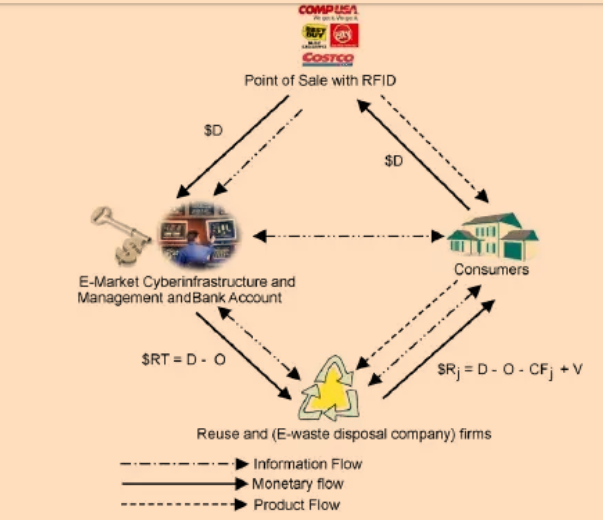
\includegraphics[width=0.7\textwidth]{one1.png}
\caption{Deposit refund system}
\end{figure}

\subsubsection{Hazardous waste transport management system}
A hazardous waste shipment system provides monitoring and control to verify the location and condition of each shipment. Two-way base stations receive status and identification signals from vehicle mounted transponders as the shipments pass by, and the base stations relay the information to a central data bank. The vehicle mounted transponders may receive data from sensors that monitor the load, and may actuate alarms or a message display for operator intervention. The three-tier system also provides notifications, and safety instructions in the event of a mishap, with the base stations relaying instructions or route changes to the vehicle mounted transponders\cite{hassett1994hazardous}.
\pagebreak
\begin{figure}[h]
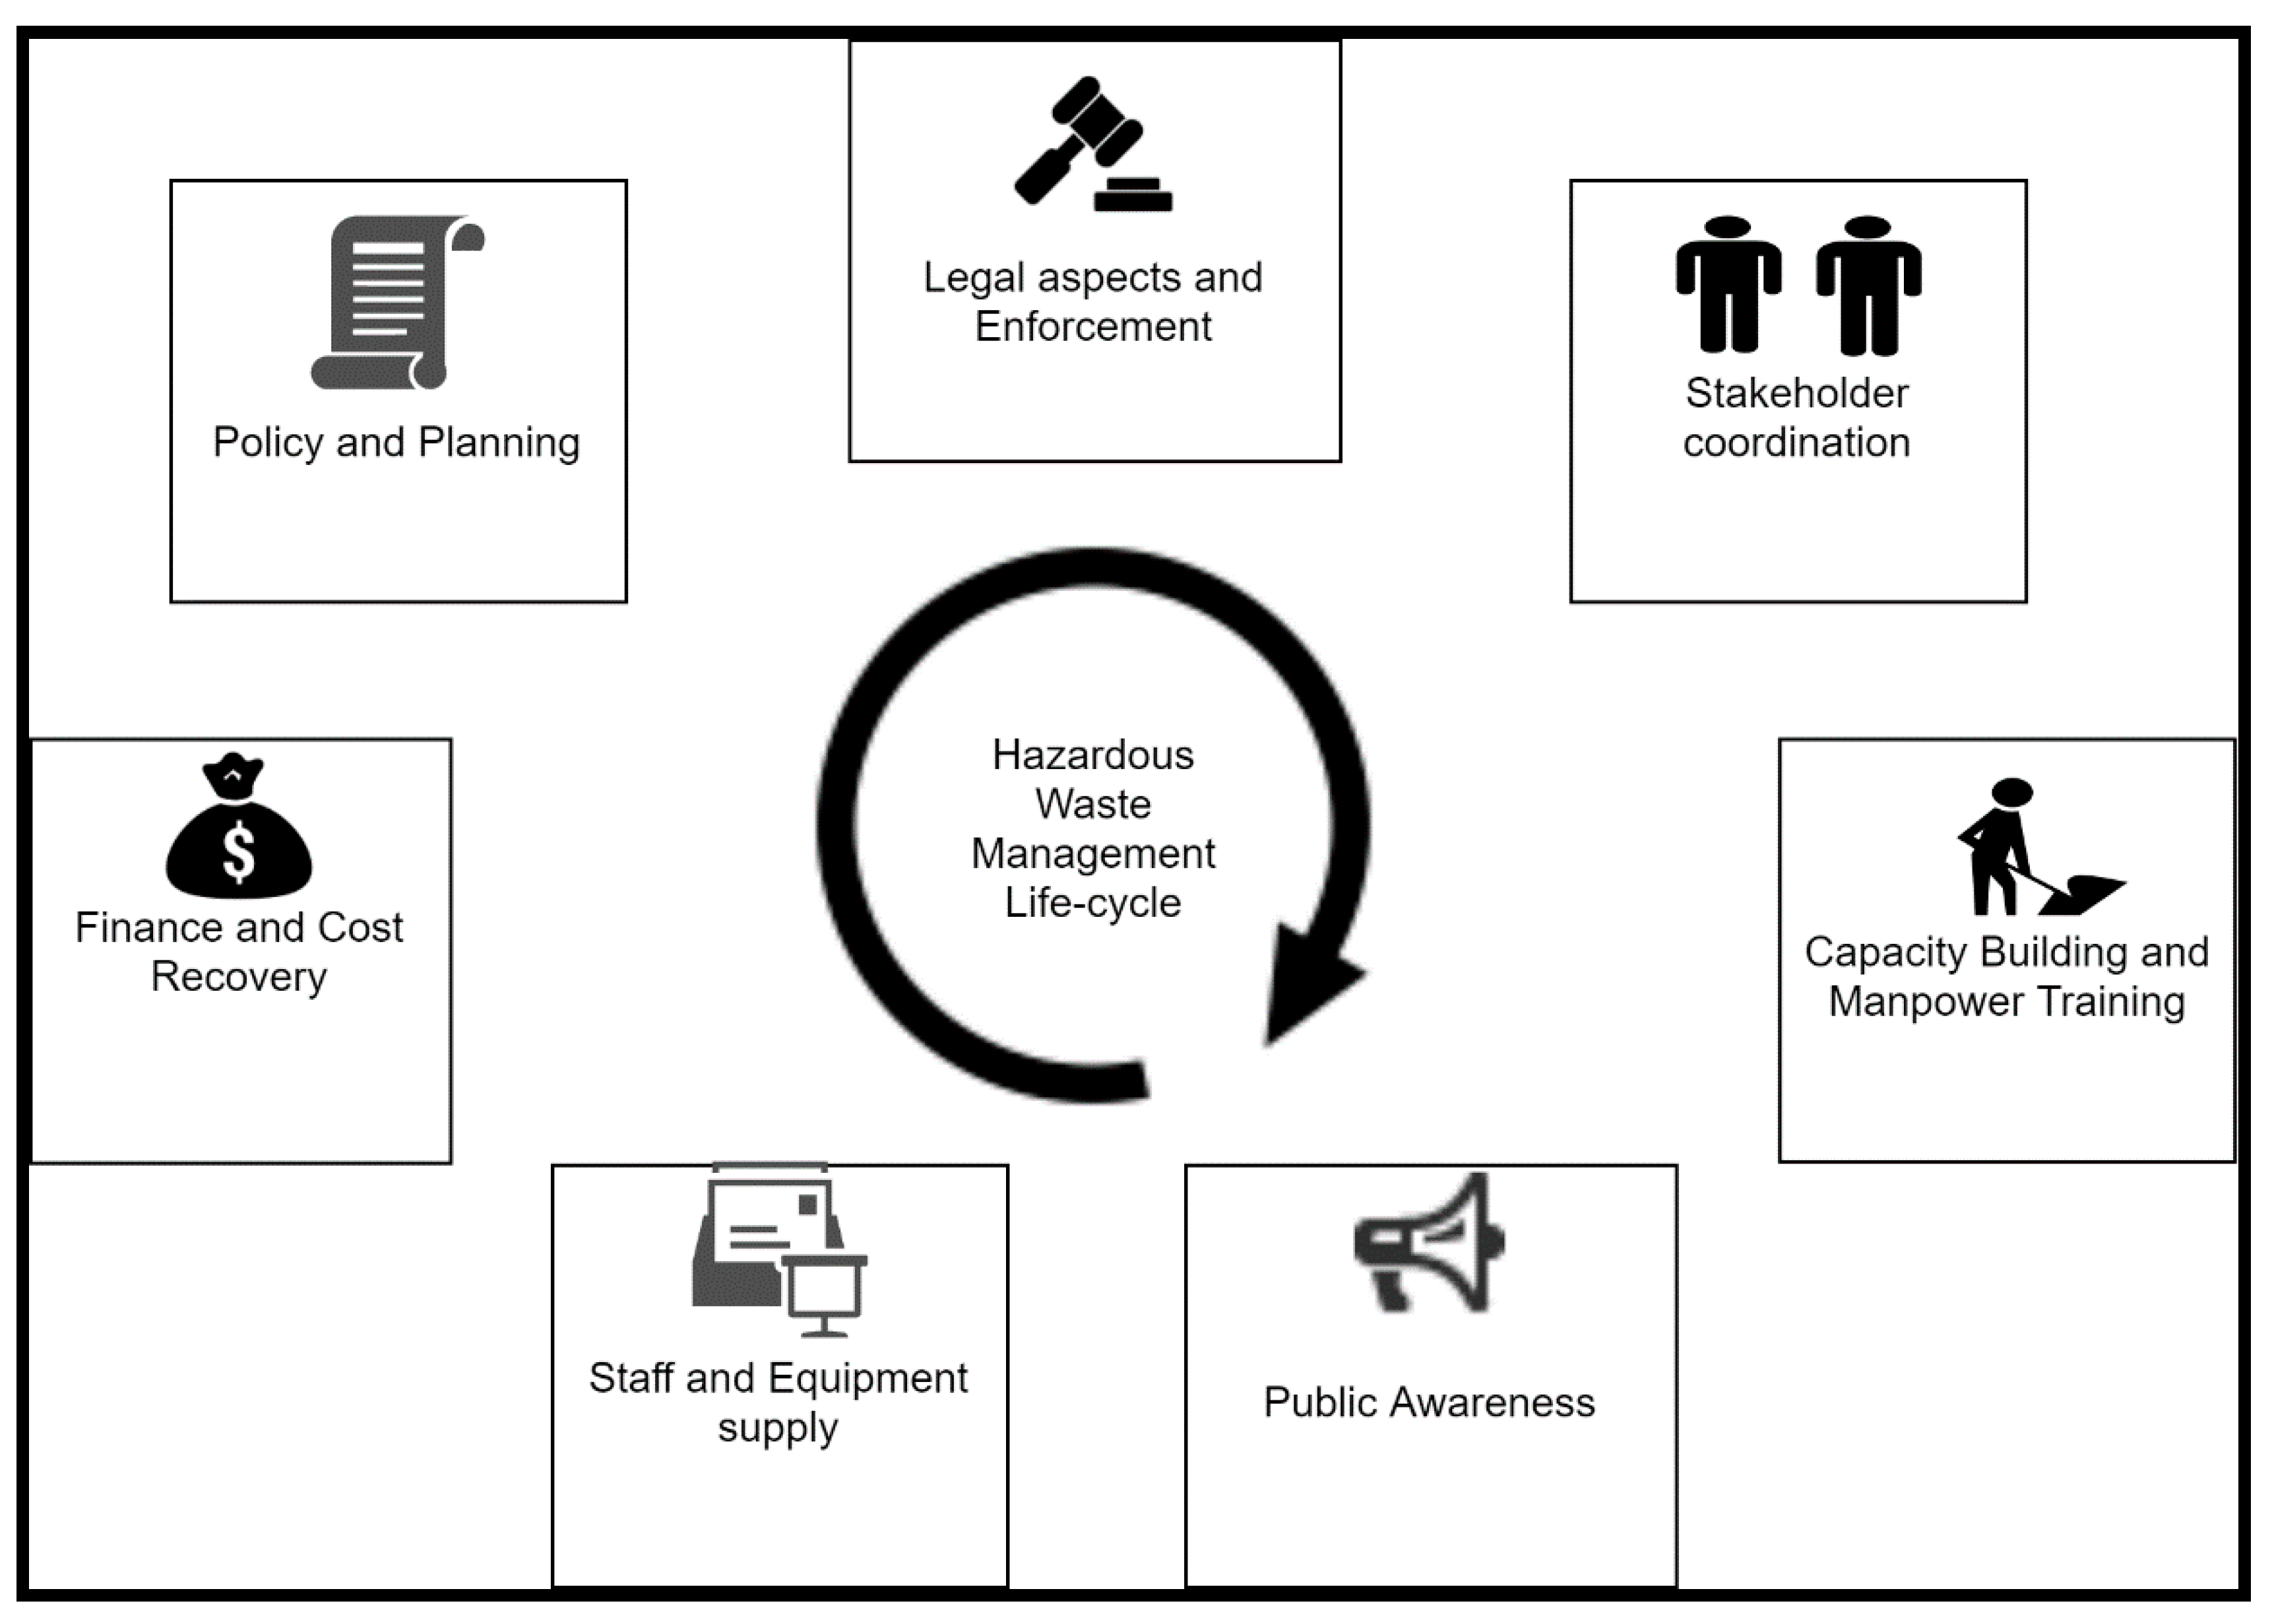
\includegraphics[width=0.8\textwidth]{recycling.png}
\caption{Hazardous waste transport management system}
\end{figure}
\subsubsection{The WEEE management system in Poland}
In Poland, the government has adopted a system that deals with a proper management and handling of E-waste materials as they are hazardous to the health of it's citizens. The system provides a collection site where the waste is collected and processed where in this case a product may find its way to the market for use till end of life while other products are recycled for the market. the system puts into consideration the leid legal regulation while cnducting this activities while at the same time putting into consideration the environmental aspects like location of proper land fills for e-waste, safe transportation and safety measures for the waste handlers.\cite{cholewa2016waste}.
\pagebreak
\begin{figure}[h]
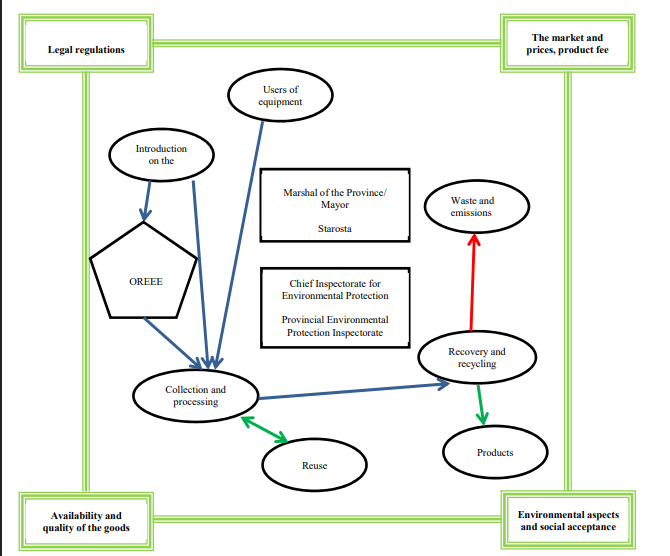
\includegraphics[width=0.9\textwidth]{poland.png}
\caption{E-waste system in Poland}
\end{figure}

\subsection{Conceptual framework}
The focus for the conceptual framework is on E-waste management that has been a common problem around the world. The framework put emphasis on five main agendas which are; the resources needed, the processes from collection to disposal, the key stakeholders who will include the municipal counsel, the producers of these devices and repair shops since they are the most affected by load overload , the sources of e-waste and finally the legal framework that will govern on how electronic waste should be handled and what role every stake holder should play. The processes that will be involve while conducting the activity of collection, transportation, recycling, disassemble, extraction, incineration and disposal will heavily rely on the availability of resources such as labor, land and capital available to facilitate this activities.
The figure bellow illustrates the actual framework for the system.
\pagebreak\begin{figure}[h]
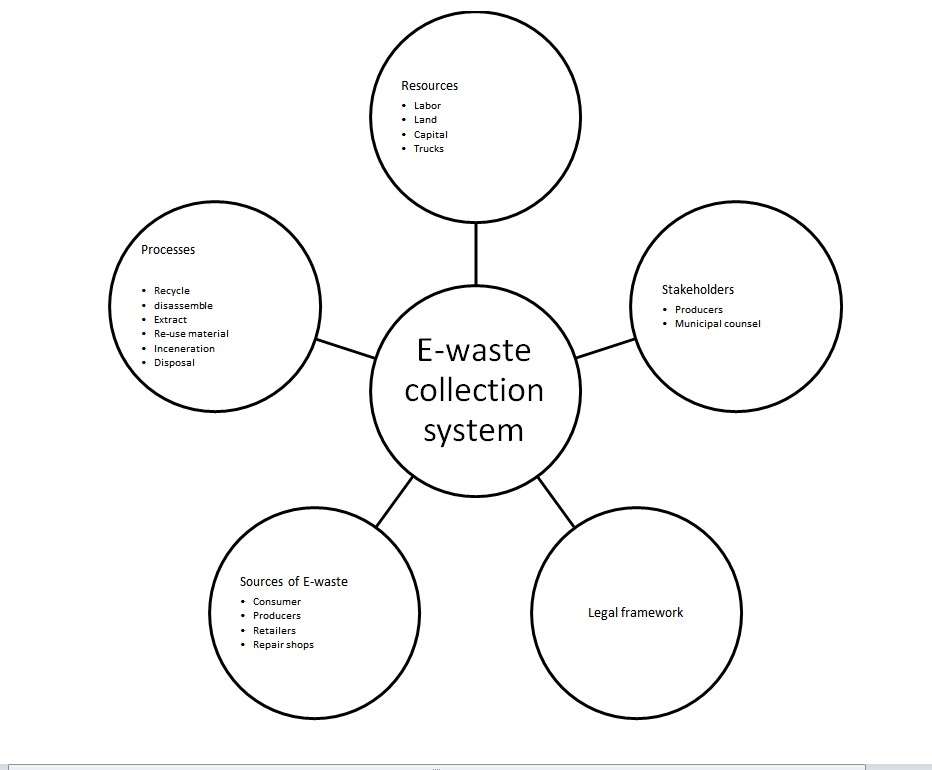
\includegraphics[width=0.9\textwidth]{one3.jpg}
\caption{proposed conceptual framework}
\end{figure}
\newpage
\section{ METHODOLOGY}
\subsection{Data sources}
The project  incorporated both the primary and secondary data sources such as the use of face to face interviews, observation by conducting site visits, use of questionnaires, journals, research articles and other publications on e-waste management in Kenya and in other countries in order to assess what needs to be done in order to manage the problem at hand.
\subsection{Collection tools}
The following data collection tools were used to obtain the data required:
\subsubsection{Face-to-Face Interview}
A face to face interview with respondents was conducted from all the concerned sectors such as the government institutions, the private institution , the non-governmental organizations  and all other parties that are affected by the current situation of E-waste management due to lack of a structured system of e-waste collection. Some of the key issues that were addressed included :
\begin{itemize}
\item The availability modes of e-waste collection.
\item Internal procedures of dealing with e-waste equipment.
\item Major sources of e-waste management within each sector.
\item The availability of policies on extended user responsibility.
\end{itemize}
\subsubsection{Questionnaires}
The project  also adapted the use of questionnaires which were divided into three sets with the first set focusing on the key stakeholders such as the customers, importers, distributers, refurbishes  and recycler. The second set will focus on the house holds that are located around the dump sites with the third set of questionnaire focusing on international bodies that are in charge of e-waste management
Some of the data collected from the adaption of this methodology included:
\begin{itemize}
\item The effects of waste disposal to member living around the dump sites.
\item Establishment of guidelines and policies on e-waste disposal.
\item The mode of e-waste collection.
\item Type of e-waste.
\item Availability of policy on extend user responsibility
\end{itemize}
\subsubsection{Observation}
Site visits were conducted especially in second hand markets and repair shops to assess and observe the current situation and made recordings based on the situation on the ground. Some of the data collected included and not limited to the following:
\begin{itemize}
\item an assesment of the kind of e-waste available.
\item Handling provedures for e-waste.
\end{itemize}
\newpage
\subsection{Architectural Framework}
\begin{figure}[h]
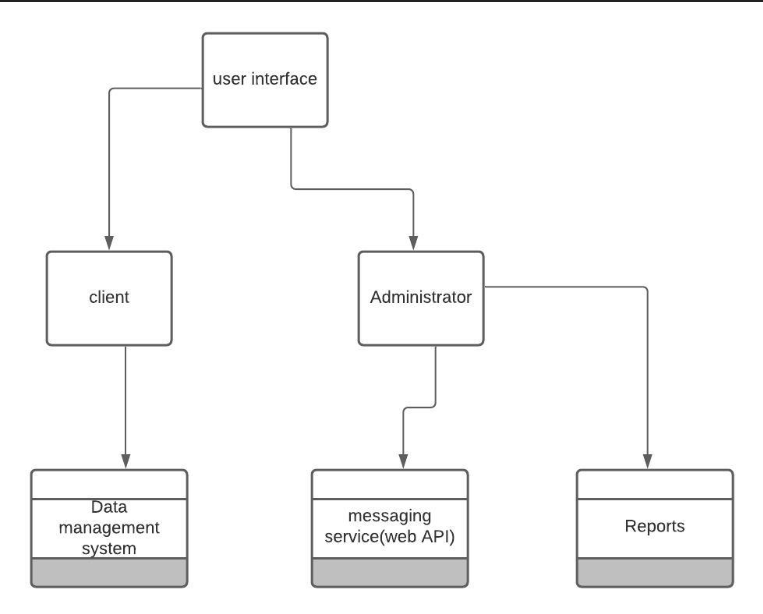
\includegraphics[width=0.9\textwidth]{archy.png}
\caption{Architectural framework}
\end{figure}
Efforts towards e-waste management are increasingly raising concerns but there are proper handling systems that have been developed to cope with the issue uniquely since e-waste management and monitoring is not systematic. The  system is web based and aim at reducing the level of e-waste. This system acts as a link between the users of the system and the recycling and disposal agencies with emphasis being put on the need for extended user responsibility policy.
From this system, the different users are able to register and login with the basic login details via the user interface. The registration details are recorded and stored in the database. When the users login to the system, they will be presented with a page from where they select the item they wish to dispose from the three main categories namely computers, laptops and computer accessories. .
\subsection{Relationship Between Conceptual Framework and Architectural Framework}
The relationship between the conceptual and architectural framework will come into practice as the stakeholder will use the user interface to make requests for collection of e-waste by giving a detailed specification of the kind of waste they want to dispose. The database will store the requests and generate the status of the requests made, the geographical locations for the pickups making it easier for the personnel in charge of collection as the system generates a pickup location.
\subsection{Project Implementation}
While implementing the project, various programing languages were  used for the various modules as illustrated bellow;
\subsubsection{User Interface}
When implementing the user interface, two programming languages were  used namely  HTML IV and CSS. This was achieved with the help of Dreamweaver which is a powerful tool for coding.
\subsubsection{Data management system}
The data management system was implemented using PHP programming
Language.PHP is an open source server side scripting language therefor apache webserver was installed to help in running PHP. In order to use apache, I installed XAMPP software package.
\subsubsection{System Database}
The system database was implemented using MySQL which is an open source relational SQL database management system which with the aid of its different APIs l facilitated in the creation, accessing, managing, searching and replicating the data.
\subsection{Testing}
\subsubsection{User Interface Testing}
The table below is a representation of the user interface. The data type for this field has been specified as string therefor the user should strictly insert values whose data type is string for the operation of login to be successful. This means that if the data type is not string, the operation will fail therefor not gaining the user access to the system.
\begin{table}[ht]
\centering
\caption{User interface testing}
\begin{tabular}{|c|c|c|c|c|}
\hline
Test & Action & Input & Results & Status \\
\hline
\hline
User login & pass string name, char(10) password & string name, password  & access granted & pass\\
User login & pass string name, char(10) password & string name, password char(13) & access denied & fail\\
User login & pass string name,char(10) password & integer name, password  & access denied & fail\\
\end{tabular}

\end{table}
\subsubsection{Data Management System Testing}
The database management from the table below represents an alert table. When a collection is conducted following a request, the system passes a string status as a job commissioned but if it is assigned a different data type as integer, the outcome will be a fail as that is not the data type that is requires for this field.
\begin{table}[ht]
\centering
\caption{Data management system testing}
\begin{tabular}{|c|c|c|c|c|}
\hline
Test & Action & Input & Results & Status \\
\hline
\hline
Alert table & pass string status &  commisioned & complate & pass\\
Alert table & pass string status &  integer value & incomplate & fail\\
\end{tabular}

\end{table}
\newpage
\subsubsection{System Database Testing}
The system database is in charge of storage, creation of tables, managing and searching for the data. In the case below, the alert tabulation is assigned a data type integer for the ID which is the primary key. The table will only accept values that are of integer data type for it to accept the data. If it is assigned a data type string, the table is bound to reject the value.
\begin{table}[ht]
\centering
\caption{System database teasting}
\begin{tabular}{|c|c|c|c|c|}
\hline
Test & Action & Input & Results & Status \\
\hline
\hline
Alert table & pass int ID &  int ID & value accepted & pass\\
Alert table & pass int ID &  string  ID & value rejected & fail\\

\end{tabular}

\end{table}
\newpage
\section{Project Implementation}
\subsection{\\Frontend software details}
The frontend of the project is developed elegantly to support a user interface that is interactive in nature and simple to use for any user.
\newline
The technology stack used for developing the front end application are as follows:
\begin{itemize}
\item HTML
\item CSS
\end{itemize}
\subsection{\\Backend software details}
The backend of the project is running on local machine and the database is connected to a local host. The database  stores/views and retrieves the details collected from each client.
The technology stack for developing backend application is: 
\begin{itemize}
\item MySQL
\item PHP
\item Apache (Xampp server)
\end{itemize}
\subsection{\\Sample screenshots of the project}
\subsubsection{\\Frontend}
\begin{itemize}
\item Home
\begin{figure}[h]
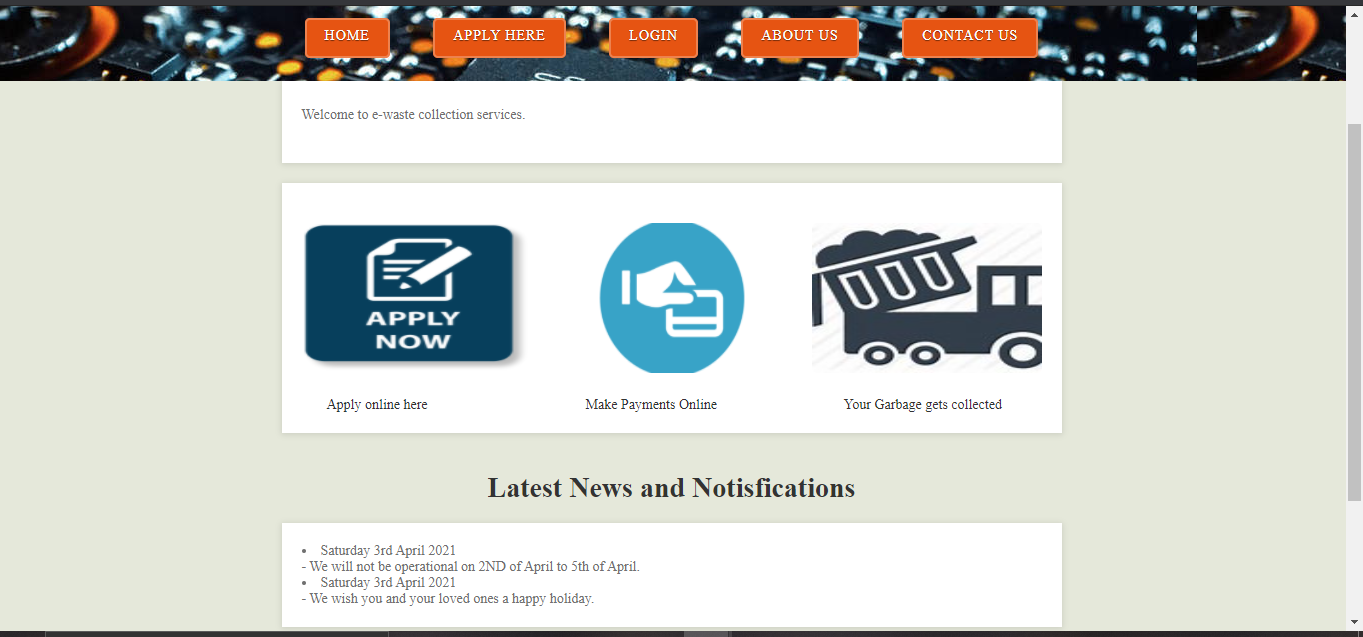
\includegraphics[width=0.8\textwidth]{Home.png}
\caption{Home page}
\end{figure}
\newpage
\item About Us
\begin{figure}[h]
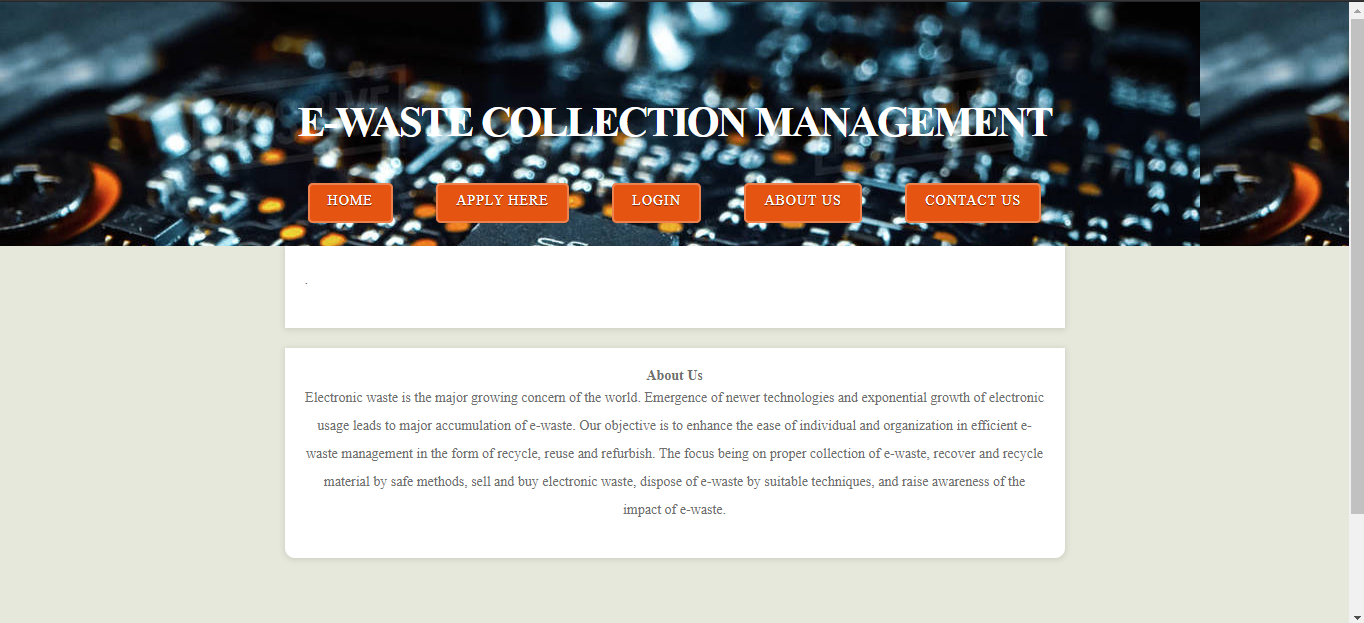
\includegraphics[width=0.8\textwidth]{About us.png}
\caption{About us}
\end{figure}
\item Contact Us
\begin{figure}[h]
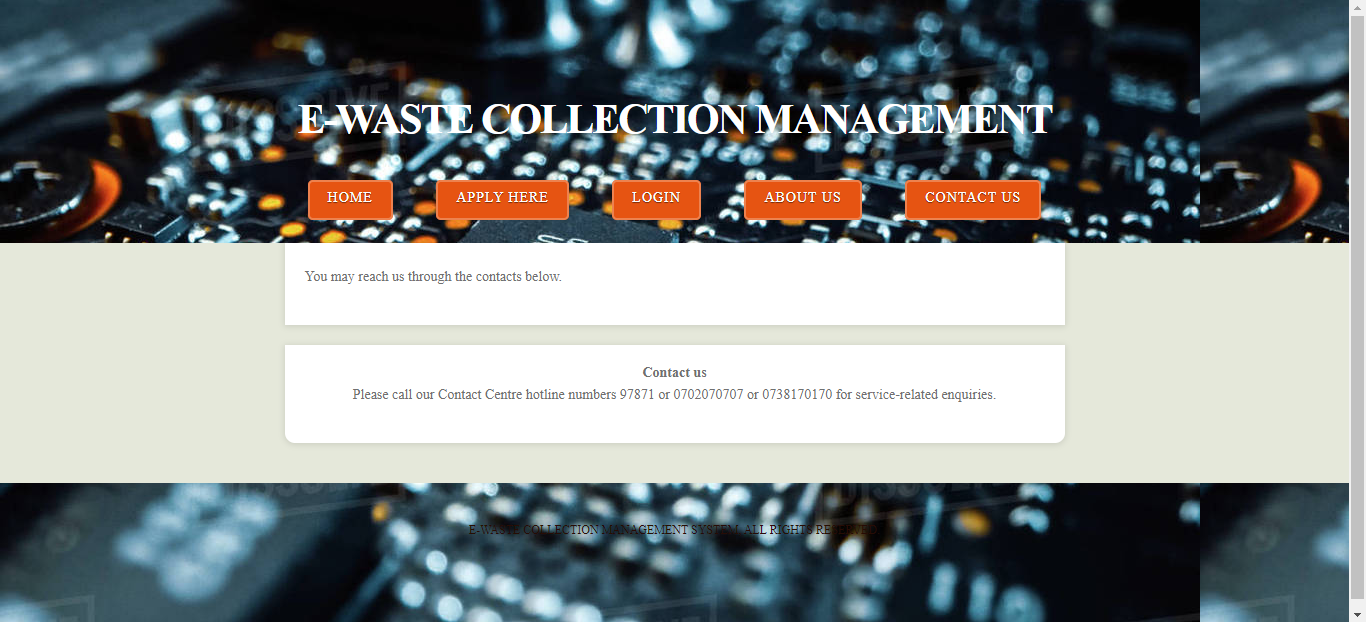
\includegraphics[width=0.8\textwidth]{ContactUs.png}
\caption{Contact Us}
\end{figure}
\newline
\newpage
\item Sign-in
\begin{figure}[h]
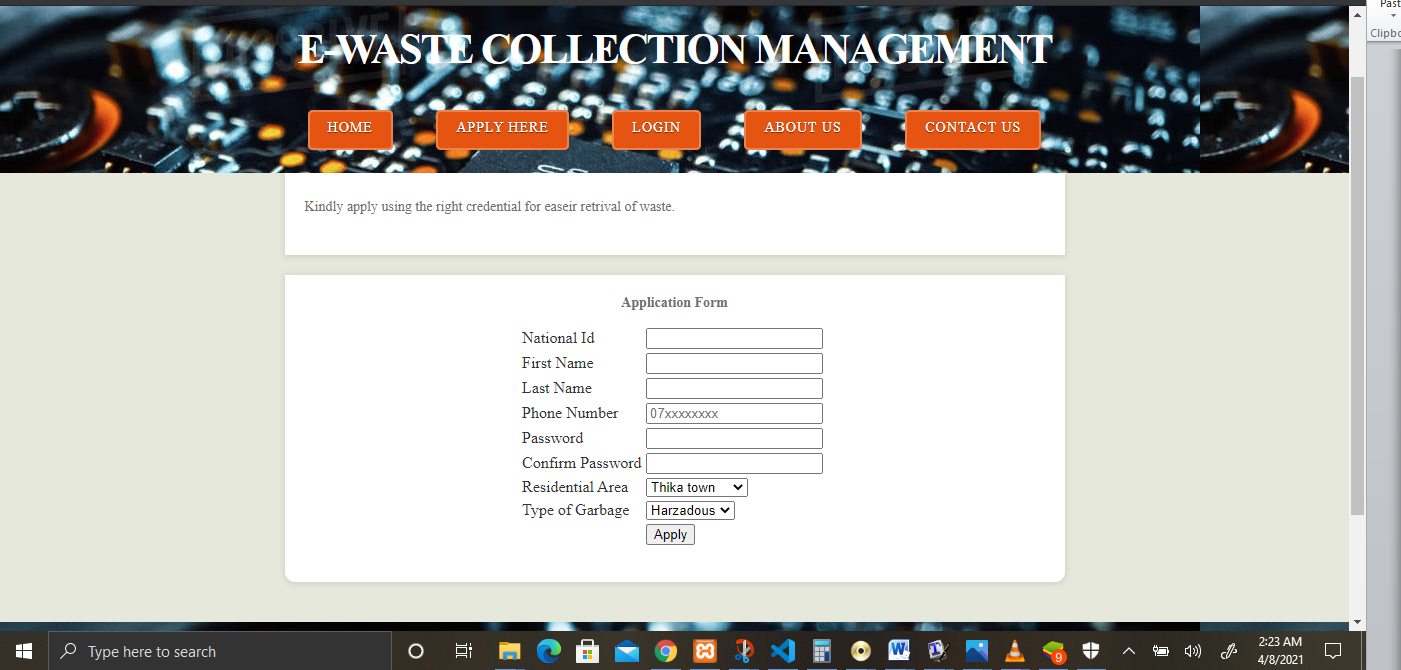
\includegraphics[width=0.8\textwidth]{Sign-in.png}
\caption{Sign in}
\end{figure}
\newline
\item Login
\begin{figure}[h]
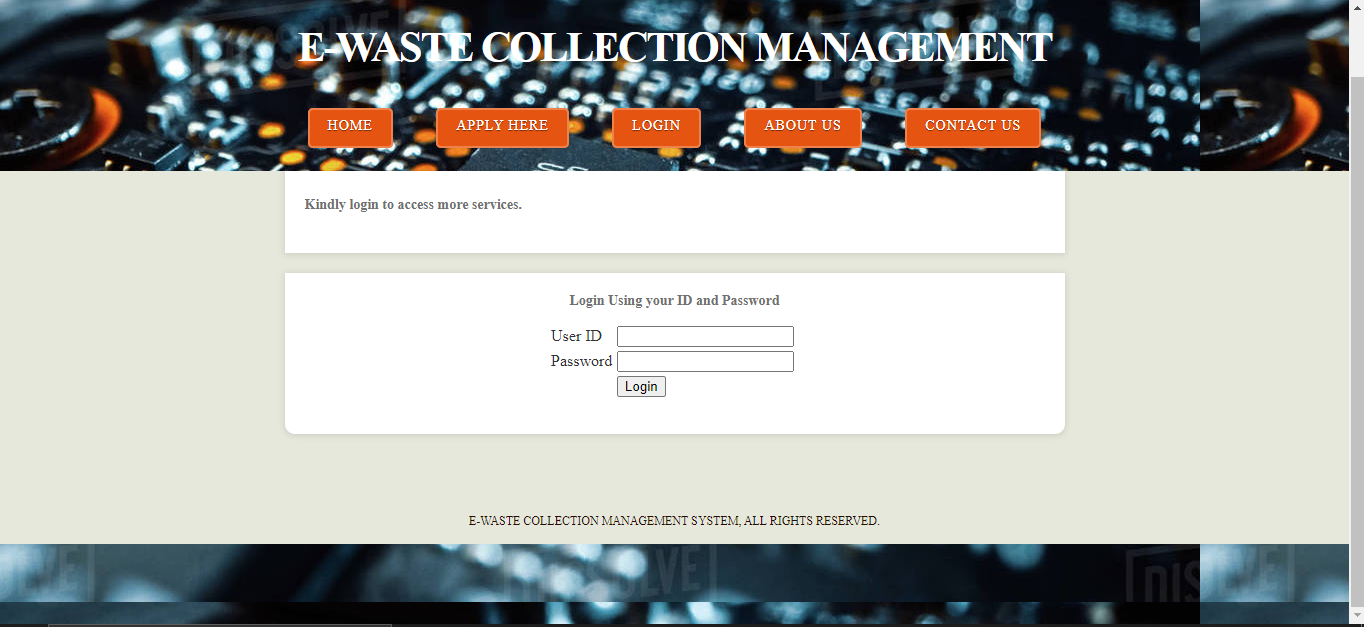
\includegraphics[width=0.8\textwidth]{Login.png}
\caption{Login Page}
\end{figure}
\newline
\newpage
\item Admin pannel
\newline
The admin can make, publish and delete notifications from this page.
\begin{figure}[h]
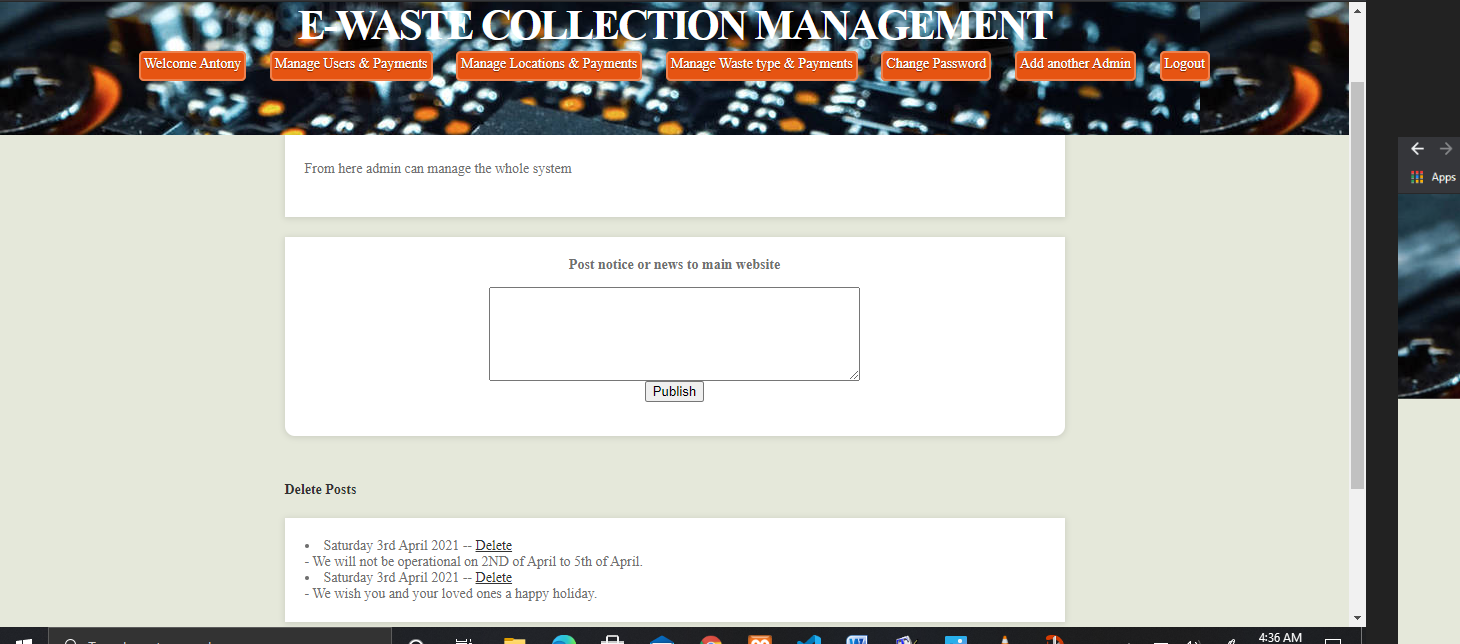
\includegraphics[width=0.8\textwidth]{Admin control.png}
\caption{Admin panel}
\end{figure}
\newline
\newpage
\item Admin manage users and payments.
\newline
The admin has the ability to view client detail along with the transactions made so that he can approve the collection of the waste upon payment.
\begin{figure}[h]
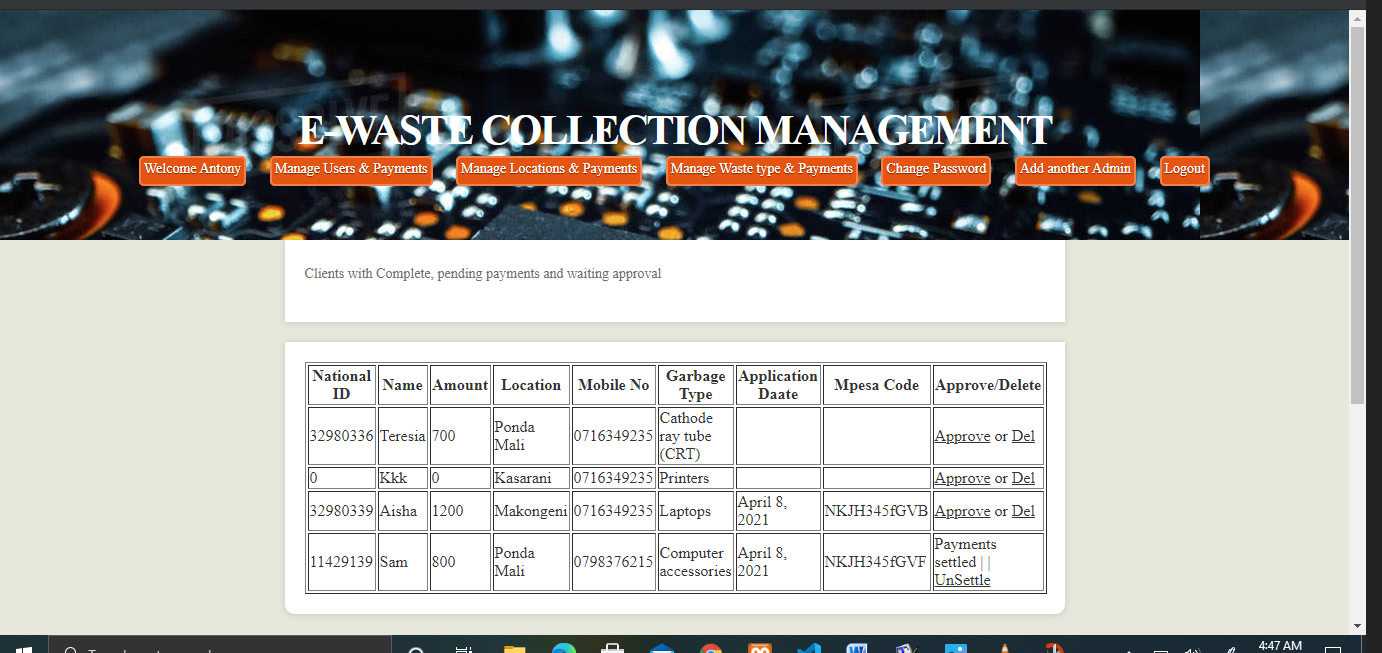
\includegraphics[width=0.8\textwidth]{fig1.png}
\caption{manage users and payments}
\end{figure}
\newline
\item Admin manage location and payments.
\newline
Here the admin can add and delete a location and also make changes on the different charges that apply to the different location charges.
\begin{figure}[h]
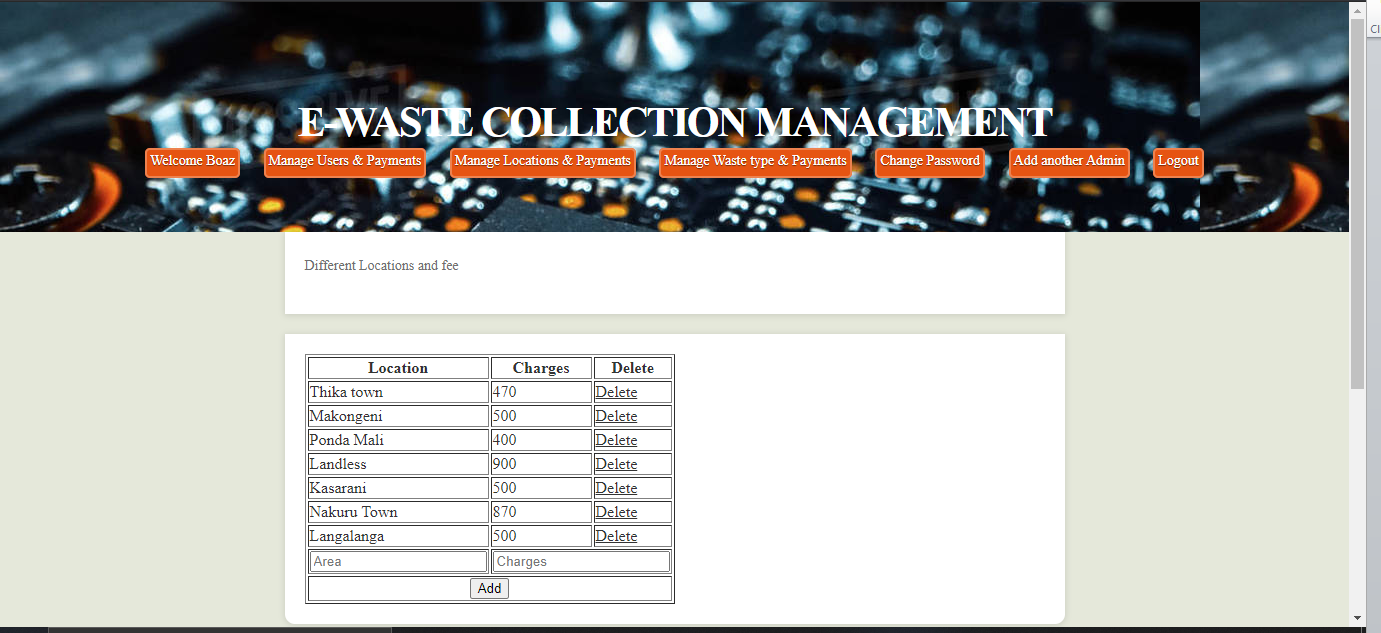
\includegraphics[width=0.8\textwidth]{fig2.png}
\caption{manage  location and payments}
\end{figure}
\newline
\newpage
\item Admin manage waste type and payment.
\newline
 The admin is able to add a waste type with its distinct price for collection. This page gives the admin the ability to change the prices for the waste along with the waste type. He/she is able to perform the functionality of update and deletion.
\begin{figure}[h]
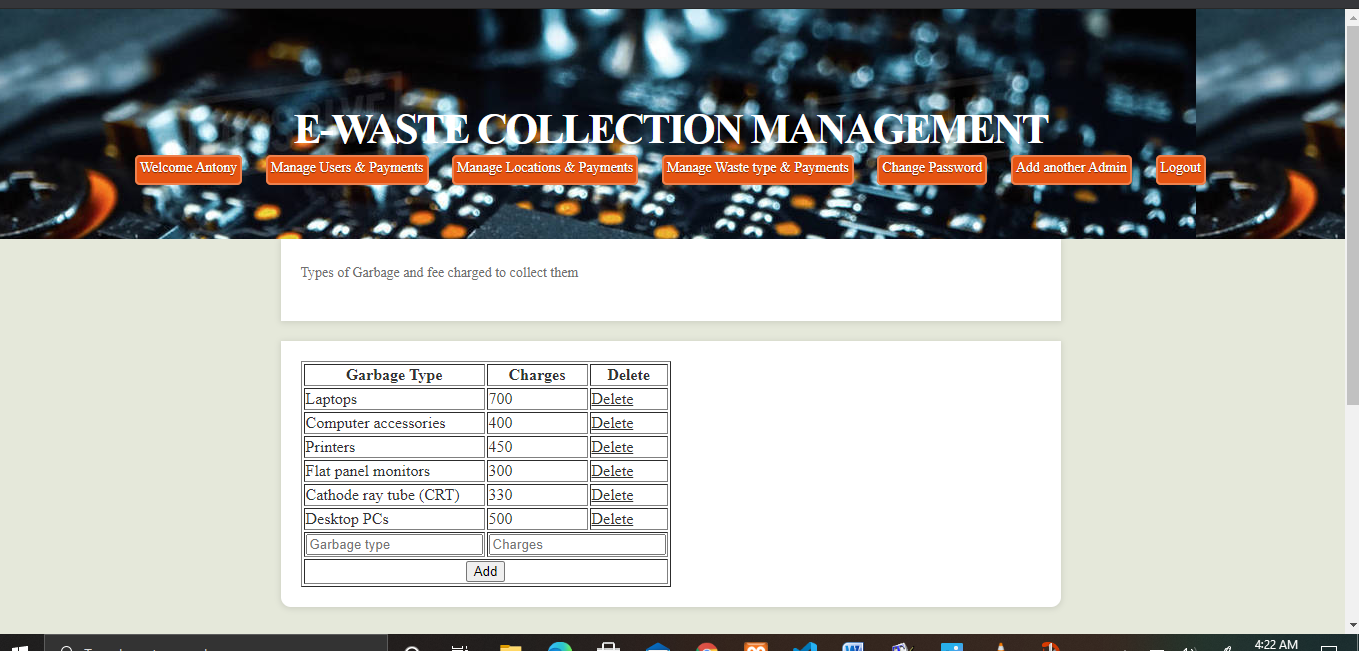
\includegraphics[width=0.8\textwidth]{fig3.png}
\caption{manage waste type and payment.}
\end{figure}
\newline
\item Admin manage password.
\newline Each admin is able to manage individual password for security purposes.
\begin{figure}[h]
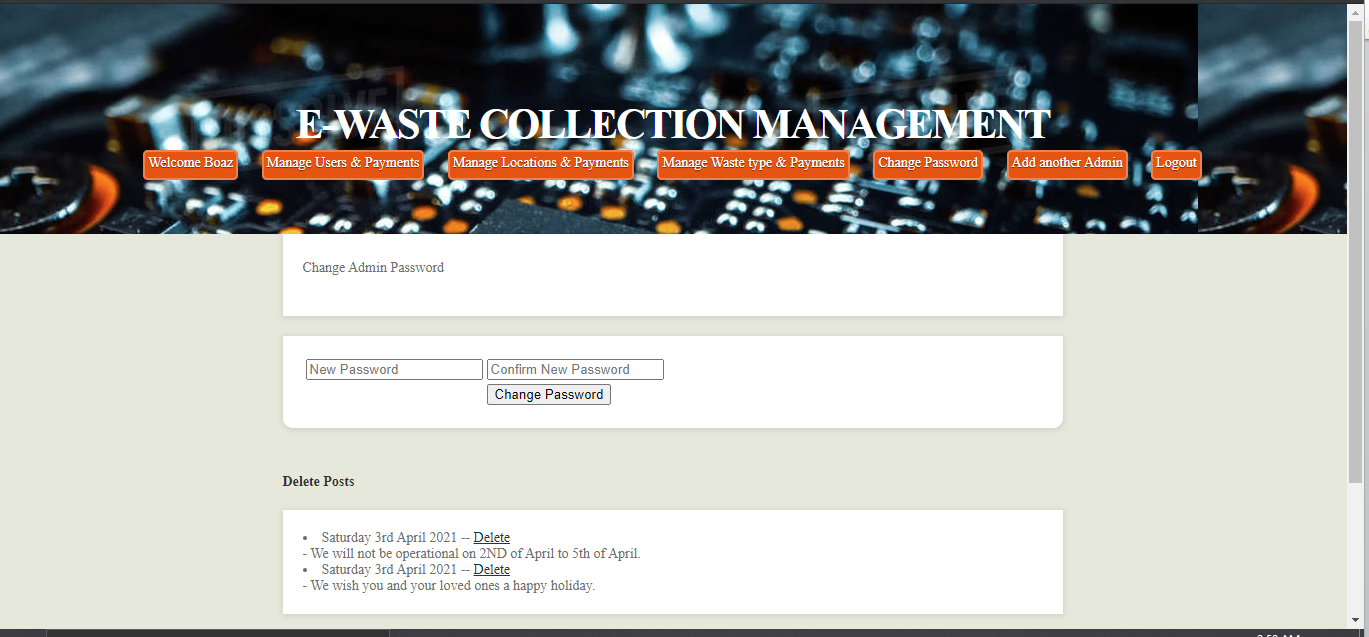
\includegraphics[width=0.8\textwidth]{fig4.png}
\end{figure}
\newline
\newpage
\item Admin manage other admins.
\newline From this page the admin is able to add or remove another admin from the system.
\begin{figure}[h]
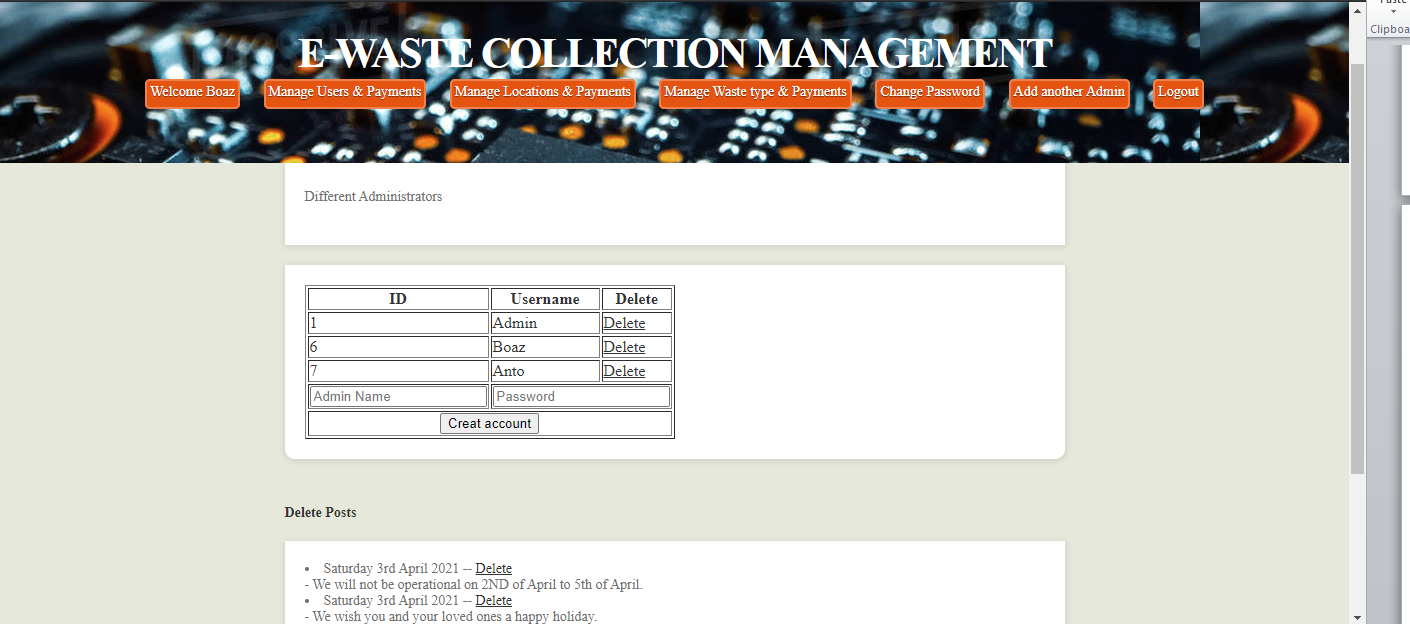
\includegraphics[width=0.8\textwidth]{fig5.png}
\caption{Manage other admins}
\end{figure}
\newline
\item Client panel.
\newline Upon login, the client gets to this page that indicate some of the details they provided during the application period.
\begin{figure}[h]
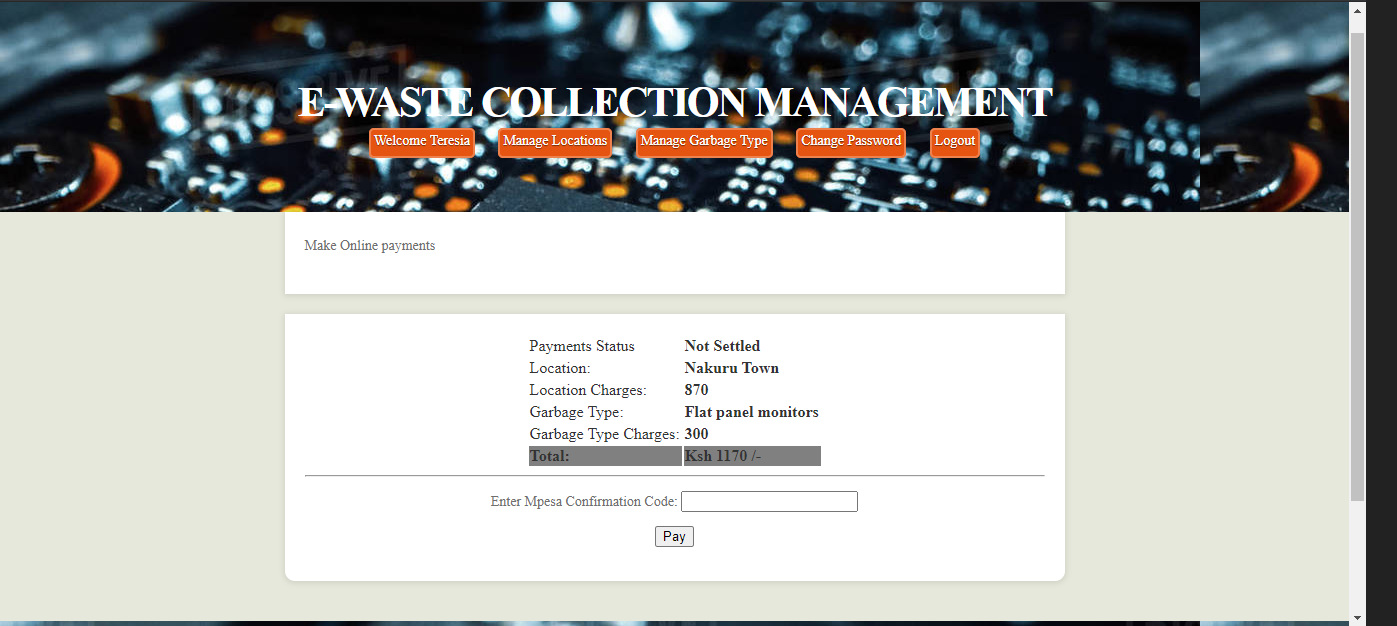
\includegraphics[width=0.8\textwidth]{fig11.png}
\caption{Client pannel.}
\end{figure}
\newline
\newpage
\item Client manage location.
\newline The client can change the location where the waste is to be picked if for one reason or the other they indicated the wrong location during the application period. This gives them the chance to revert to a location of their choice.
\begin{figure}[h]
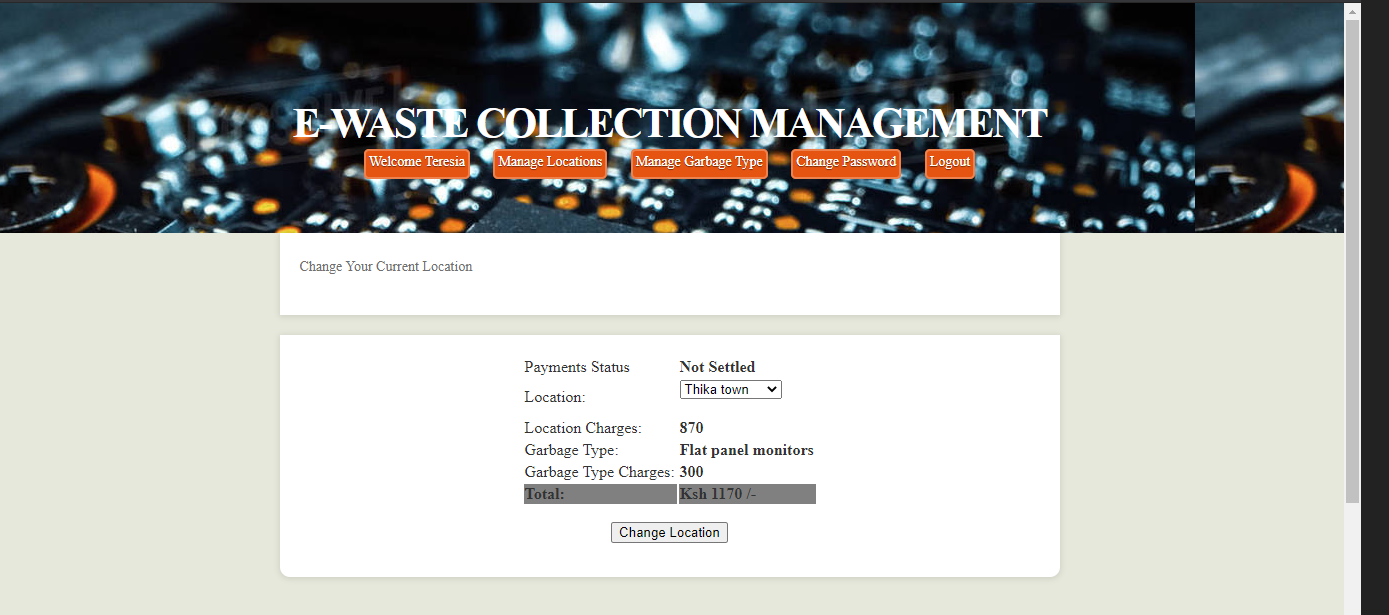
\includegraphics[width=0.8\textwidth]{fig12.png}
\caption{Manage location}
\end{figure}
\newline
\item Client manage waste type.
\newline From here the client can edit the waste type as indicated in the differences in the prices on fig18 and fig19 respectively with the change in amount paid per the waste type.
\begin{figure}[h]
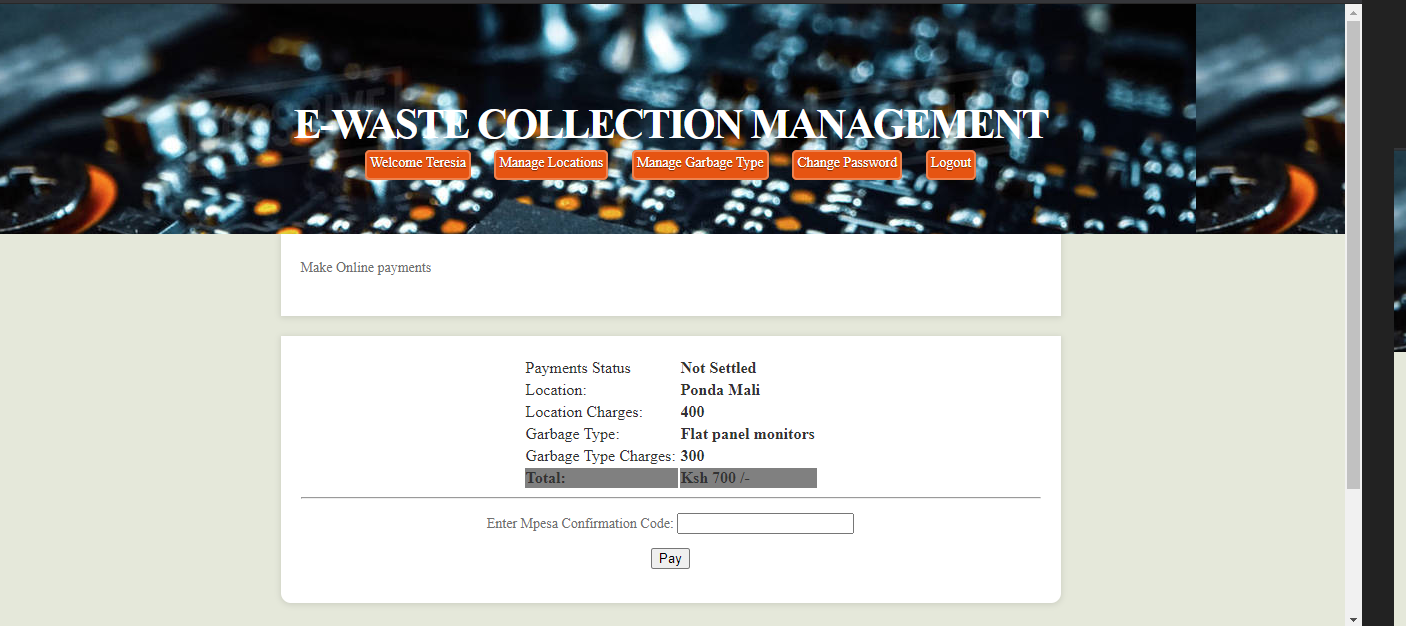
\includegraphics[width=0.8\textwidth]{fig13.png}
\caption{Client manage waste type}
\end{figure}
\begin{figure}[h]
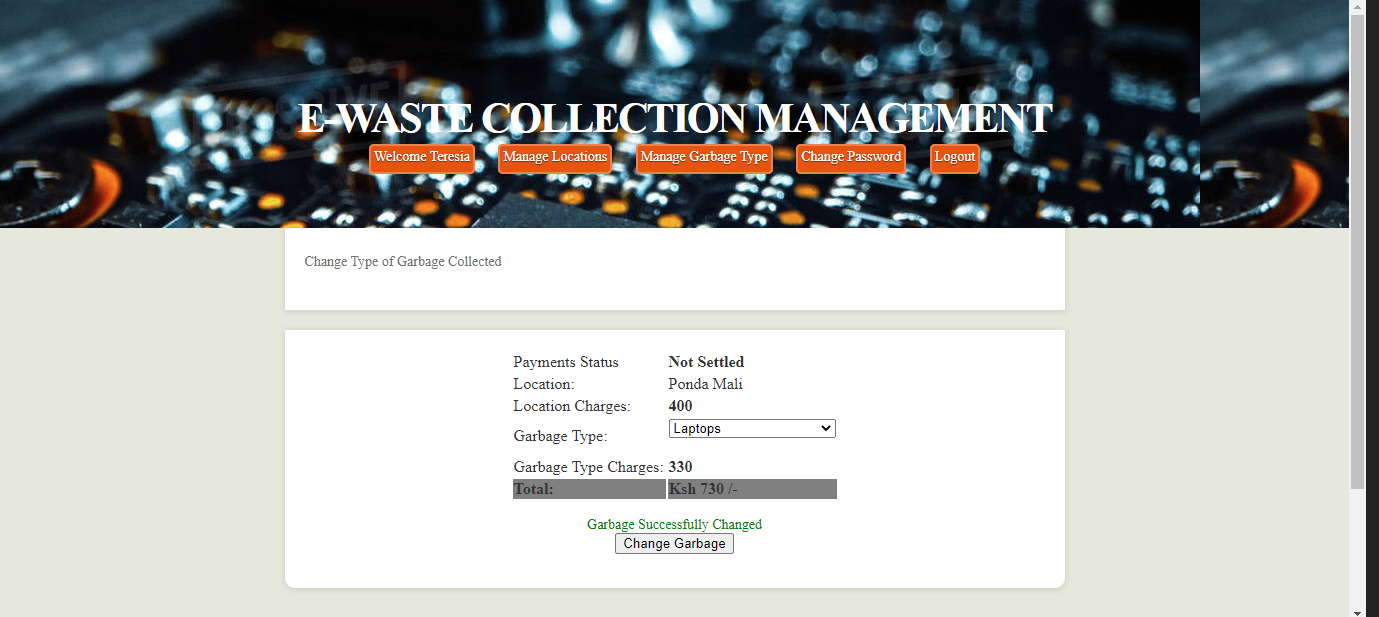
\includegraphics[width=0.8\textwidth]{fig14.png}
\caption{Client change waste type successfully}
\end{figure}
\newline
\newpage
\item Client manage password.
\newline The client has the ability to change the passwords
\begin{figure}[h]
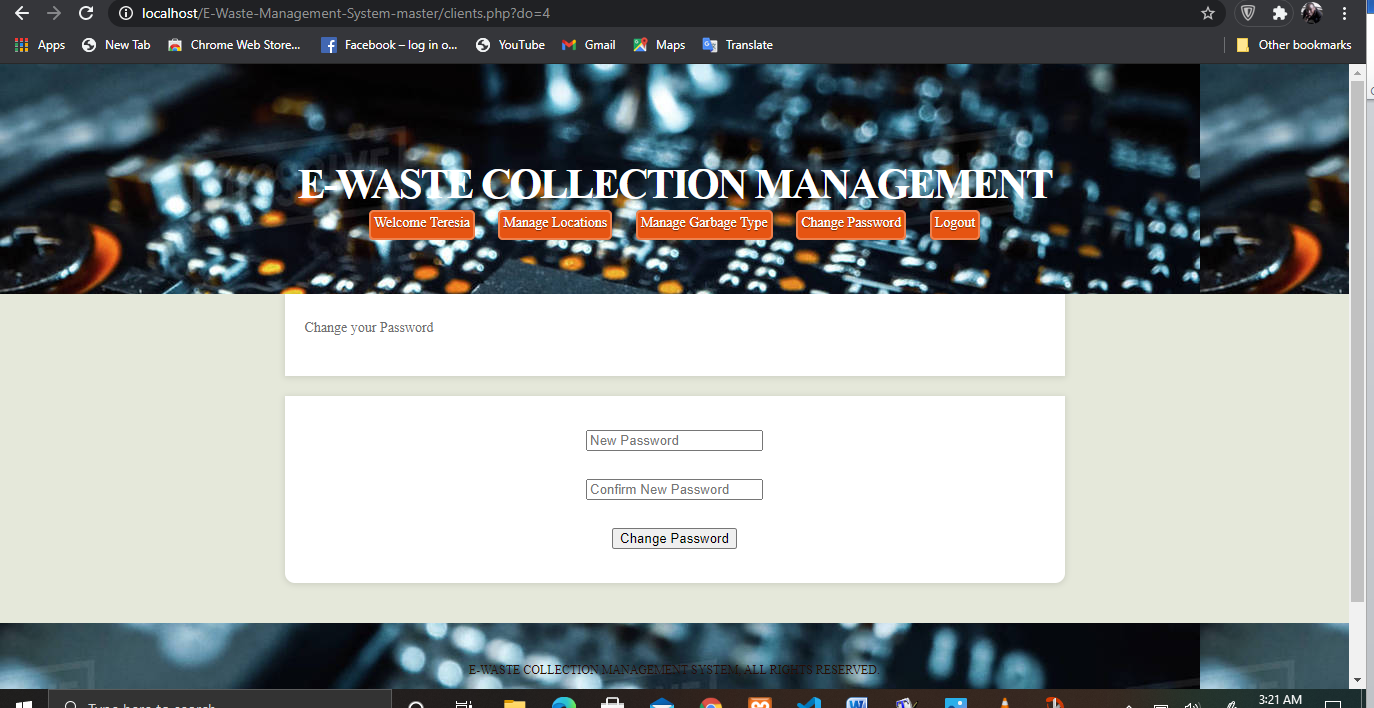
\includegraphics[width=0.8\textwidth]{fig15.png}
\caption{Client manage password}
\end{figure}
\newpage
\subsubsection{\\Backend database structure}
\item Admin table.
\begin{figure}[h]
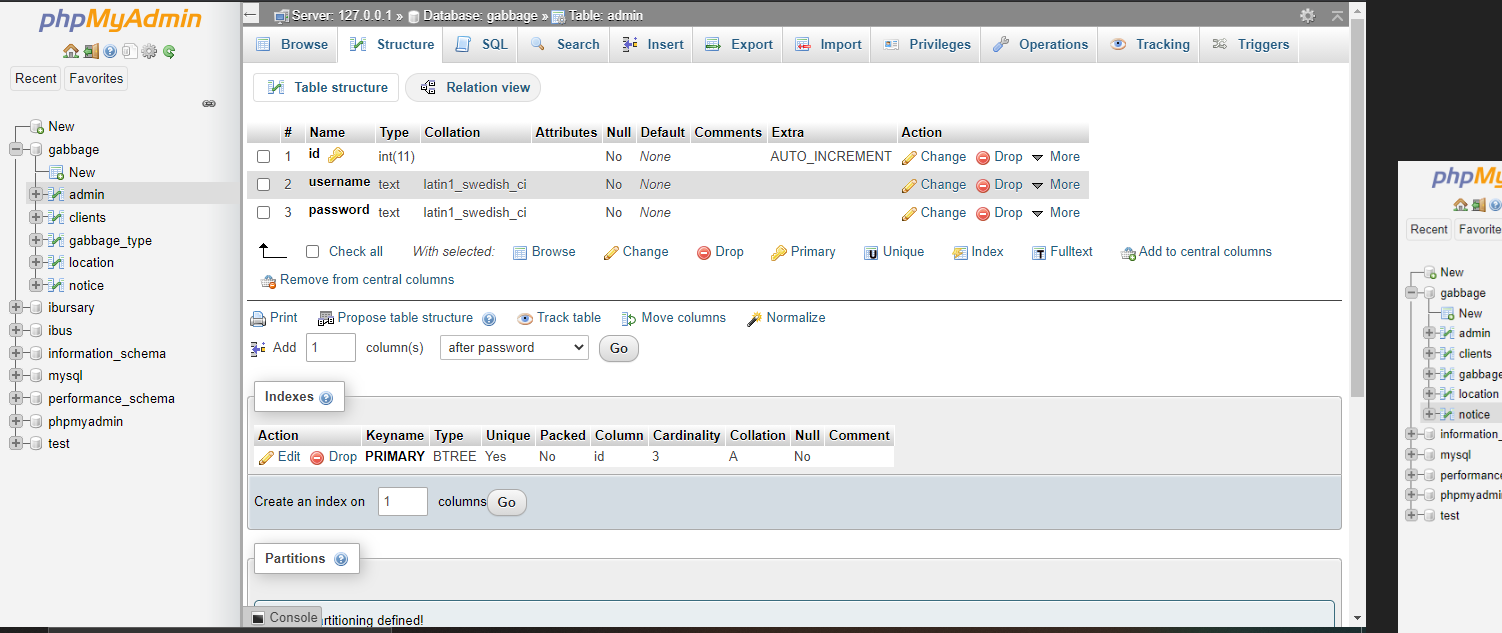
\includegraphics[width=0.8\textwidth]{Admin.png}
\end{figure}
\item Client table.
\begin{figure}[h]
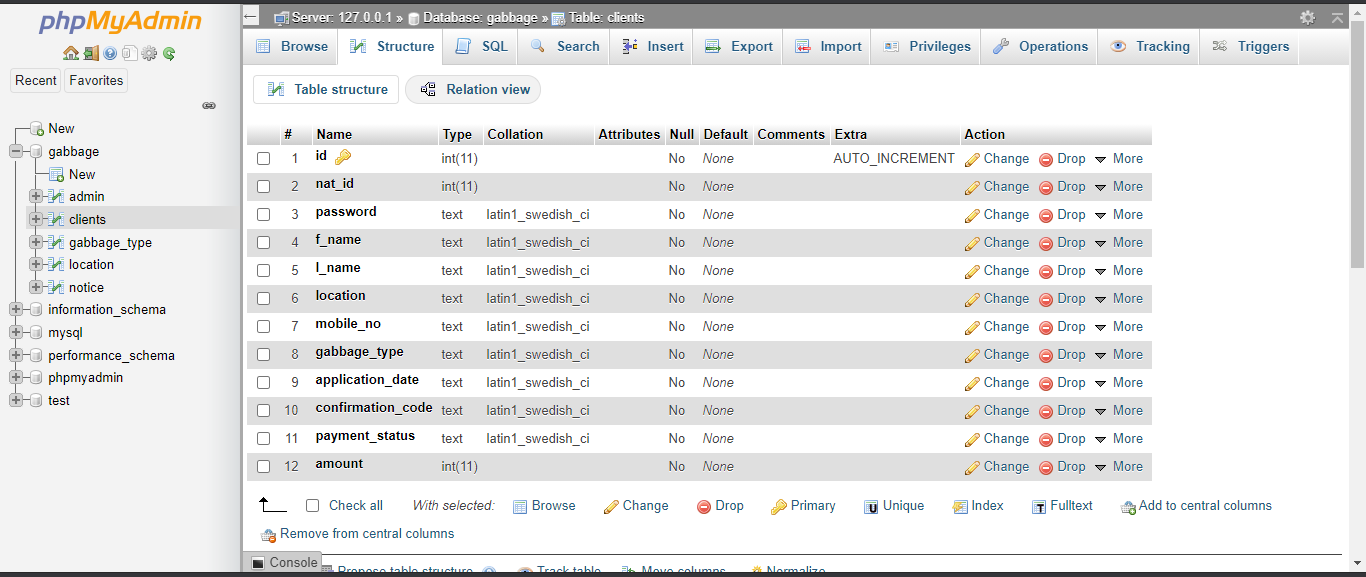
\includegraphics[width=0.8\textwidth]{Client.png}
\end{figure}
\newpage
\item Garbage type table.
\begin{figure}[h]
\includegraphics[width=0.8\textwidth]{gabbageType.png}
\end{figure}
\item Location table.
\begin{figure}[h]
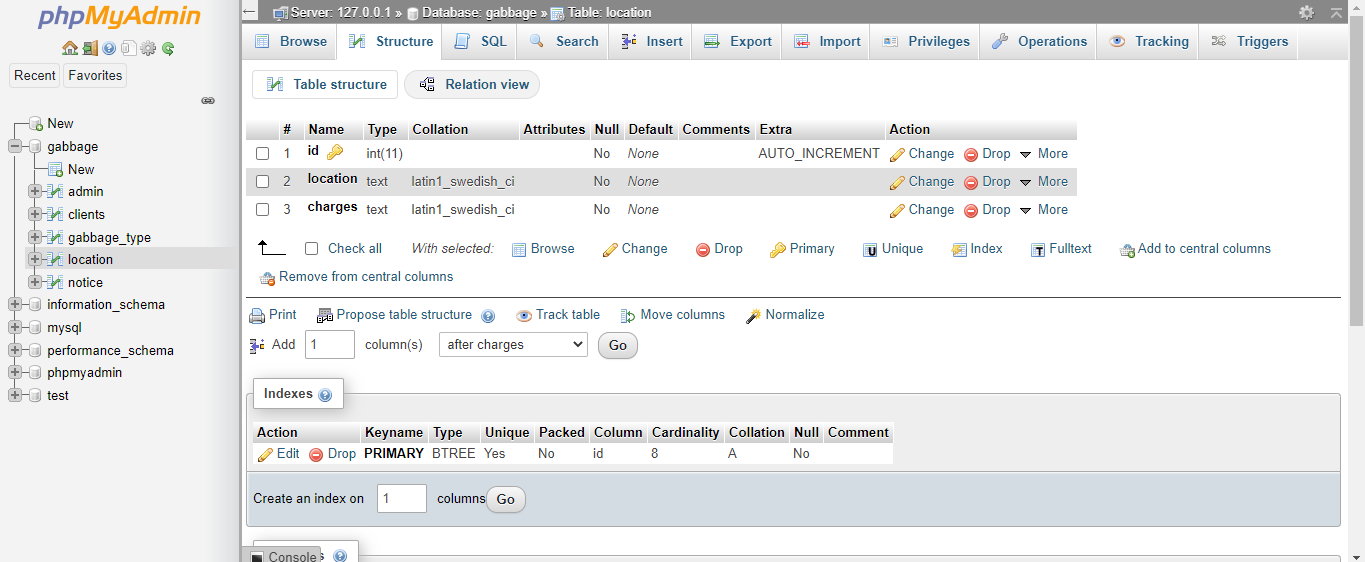
\includegraphics[width=0.8\textwidth]{Location.png}
\end{figure}
\item Notice table.
\begin{figure}[h]
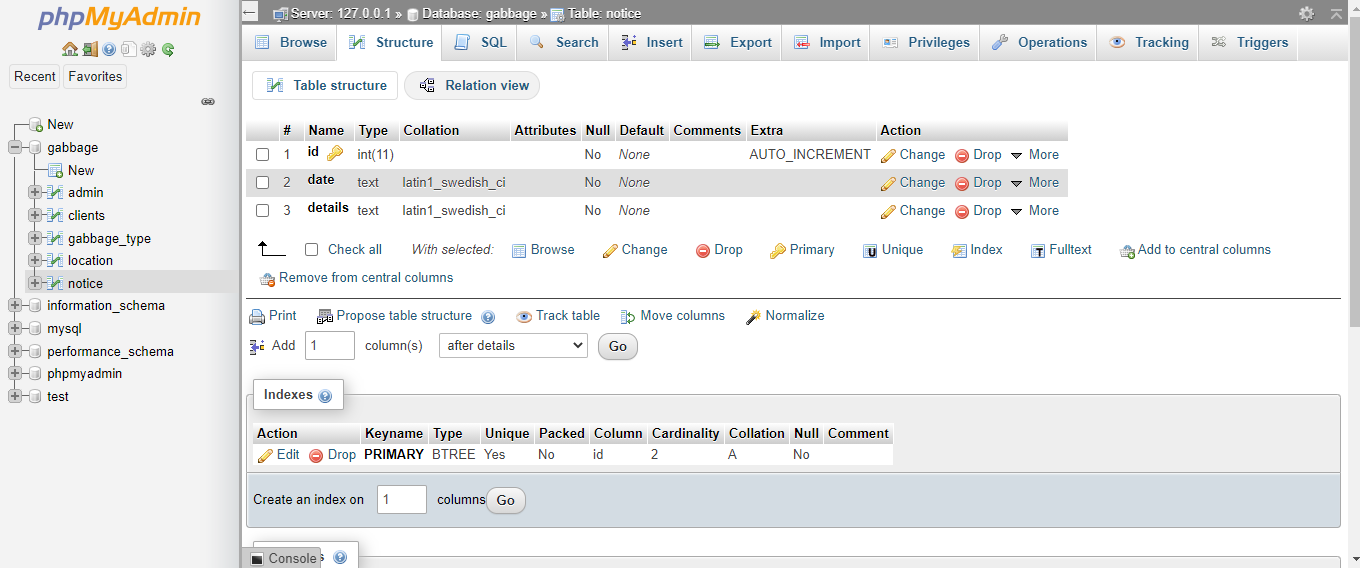
\includegraphics[width=0.8\textwidth]{Notice.png}
\end{figure}
\end{itemize}
\newpage
\subsection{\\System codes}
\begin{itemize}
\item Home
\begin{figure}[h]
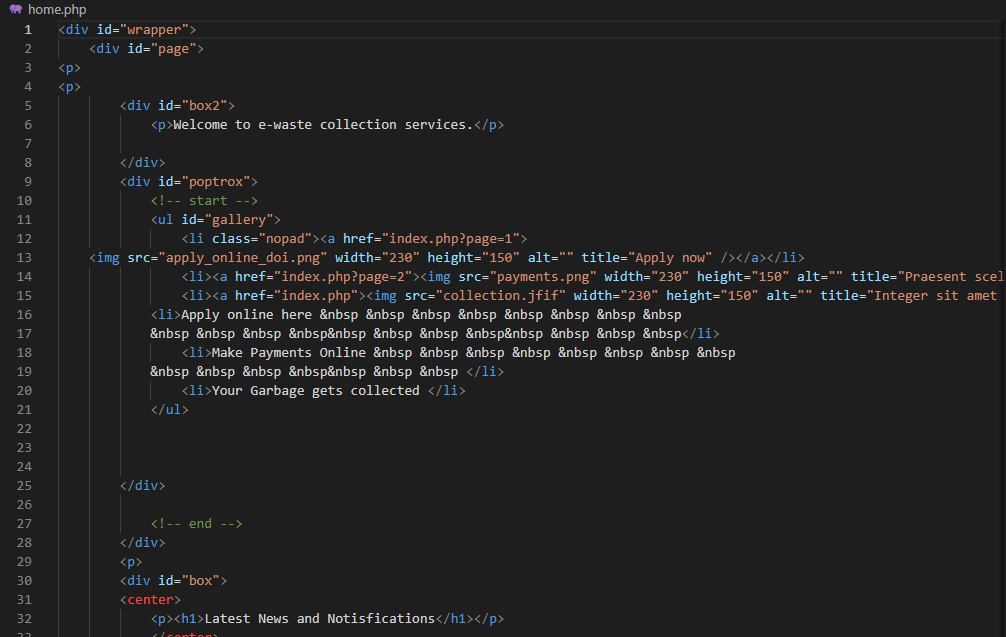
\includegraphics[width=0.8\textwidth]{Home1.png}
\end{figure}
\begin{figure}[h]
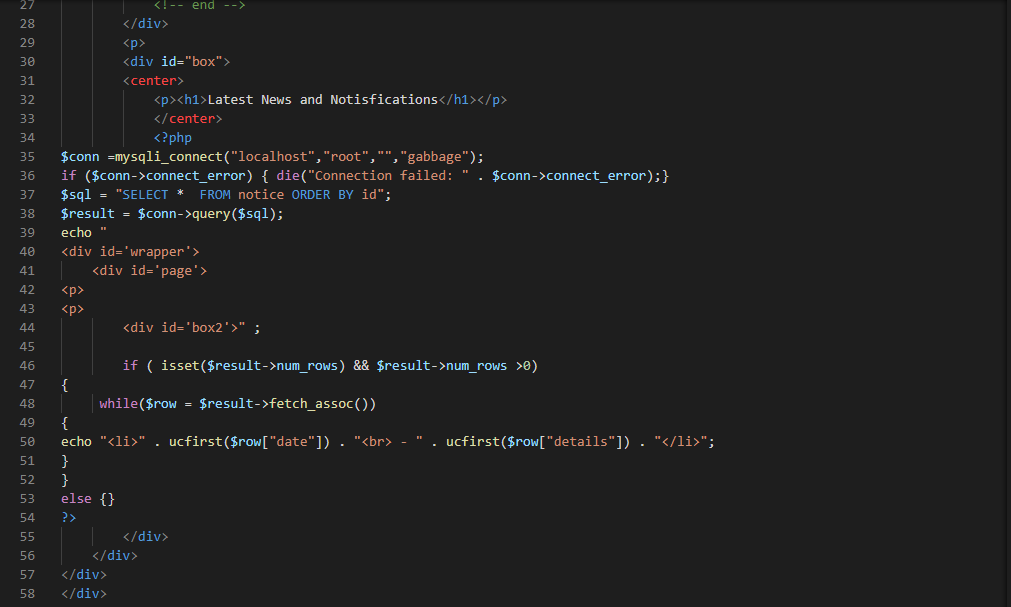
\includegraphics[width=0.8\textwidth]{Home2.png}
\end{figure}
\newpage
\item About us
\begin{figure}[h]
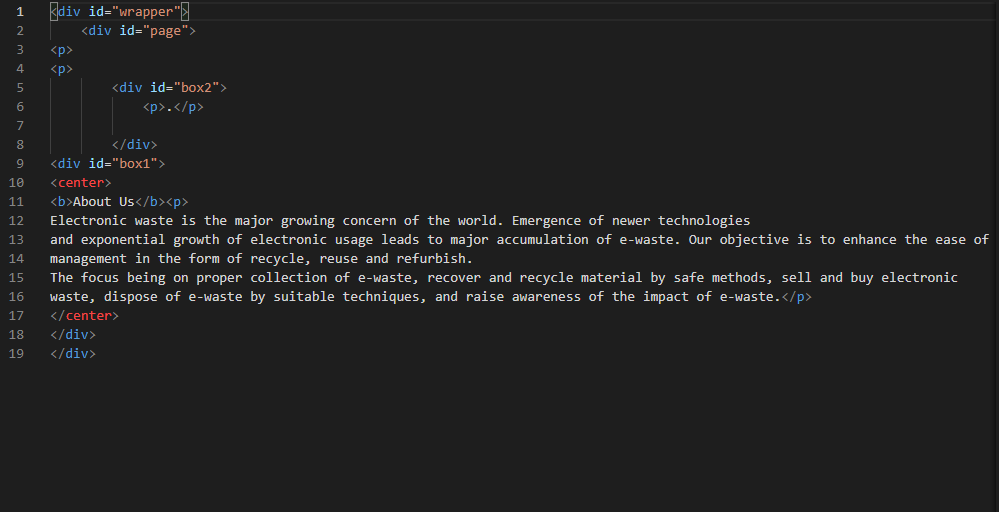
\includegraphics[width=0.8\textwidth]{About.png}
\end{figure}
\item Contact us
\begin{figure}[h]
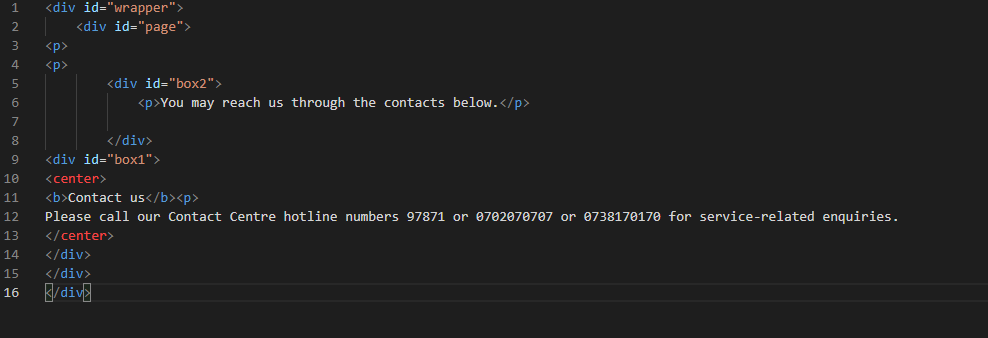
\includegraphics[width=0.8\textwidth]{contact.png}
\end{figure}
\newpage
\item Application
\begin{figure}[h]
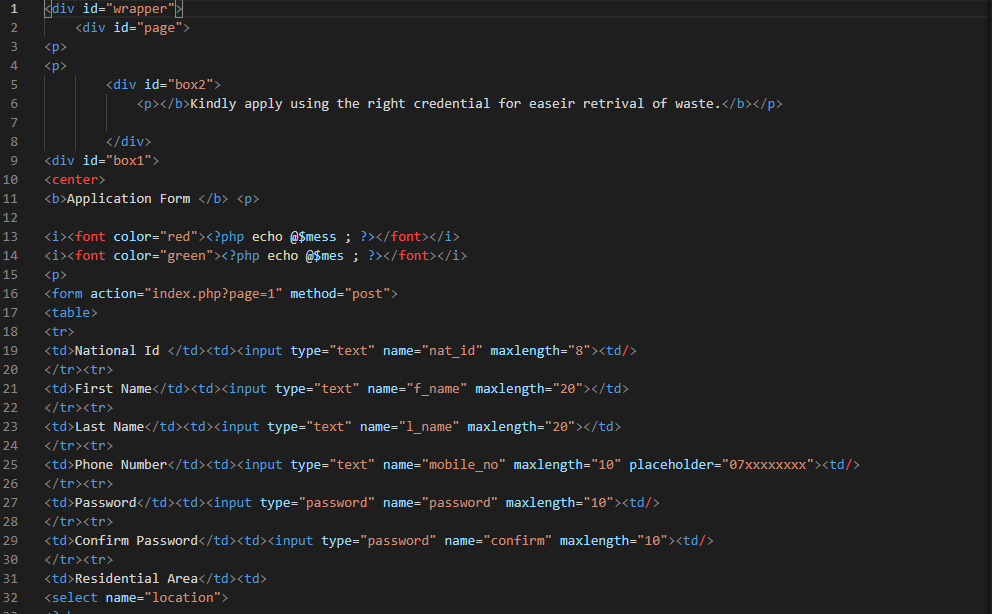
\includegraphics[width=0.8\textwidth]{ap1.png}
\end{figure}
\begin{figure}[h]
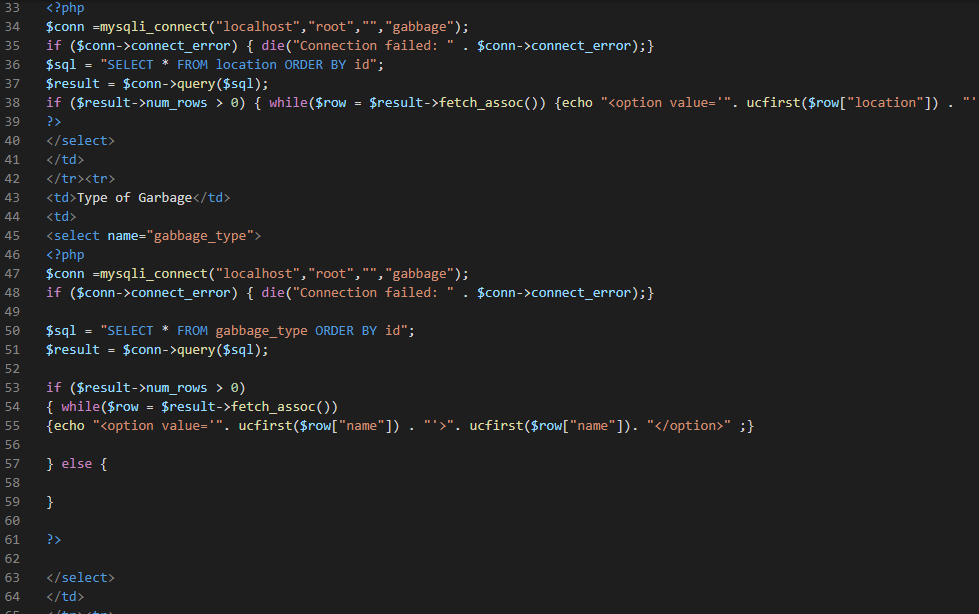
\includegraphics[width=0.8\textwidth]{ap2.png}
\end{figure}
\begin{figure}[h]
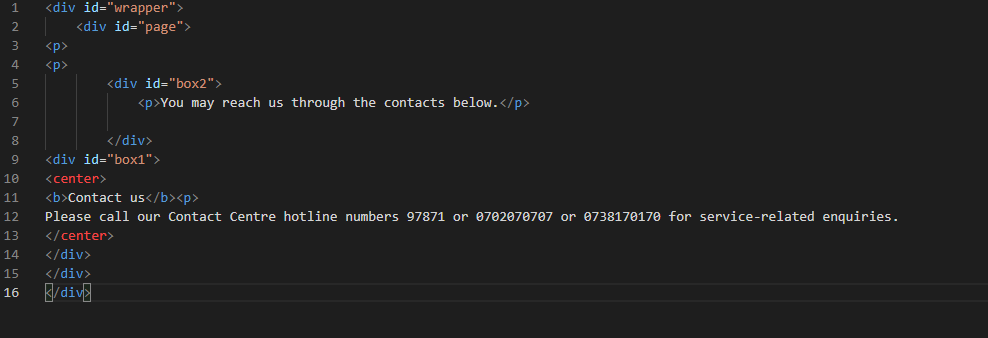
\includegraphics[width=0.8\textwidth]{ap3.png}
\end{figure}
\newpage
\item Login
\begin{figure}[h]
\includegraphics[width=0.8\textwidth]{Log1.png}
\end{figure}
\newpage
\item Admin dashboard
\begin{figure}[h]

\includegraphics[width=0.6\textwidth]{ad1.png}
\end{figure}
\begin{figure}[h]
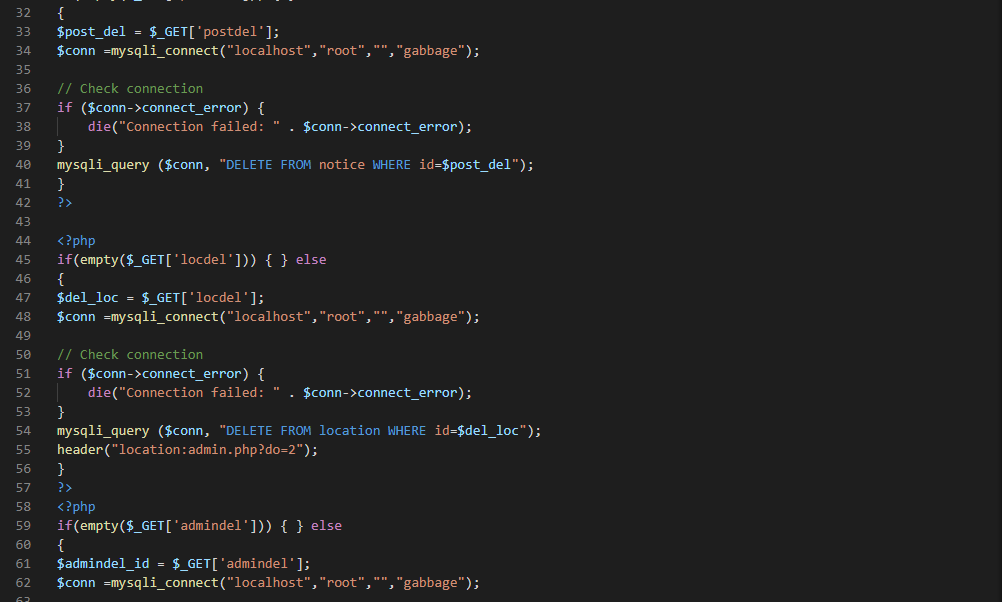
\includegraphics[width=0.6\textwidth]{ad2.png}
\end{figure}
\begin{figure}[h]
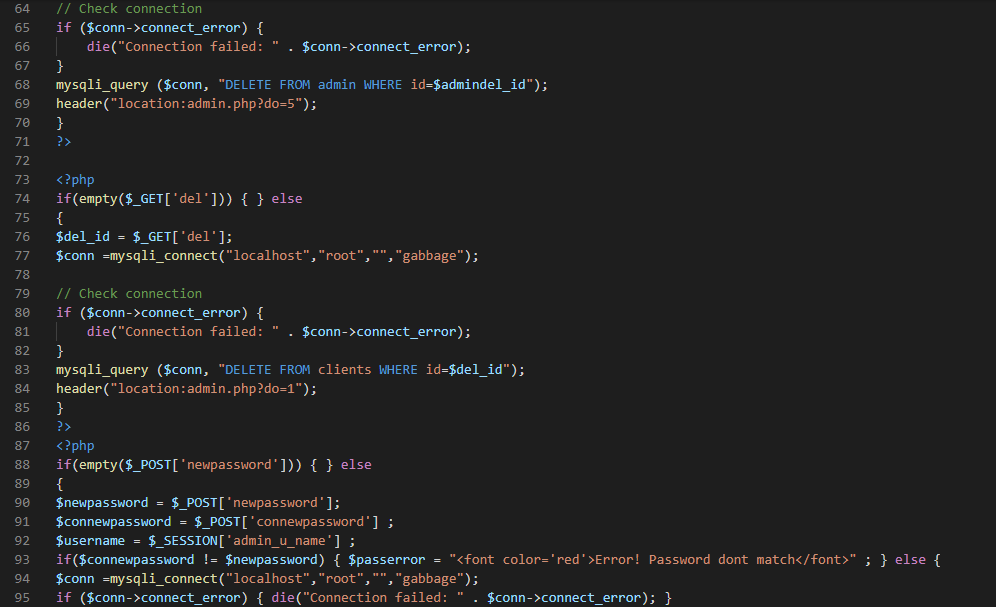
\includegraphics[width=0.6\textwidth]{ad3.png}
\newpage
\end{figure}
\begin{figure}[h]
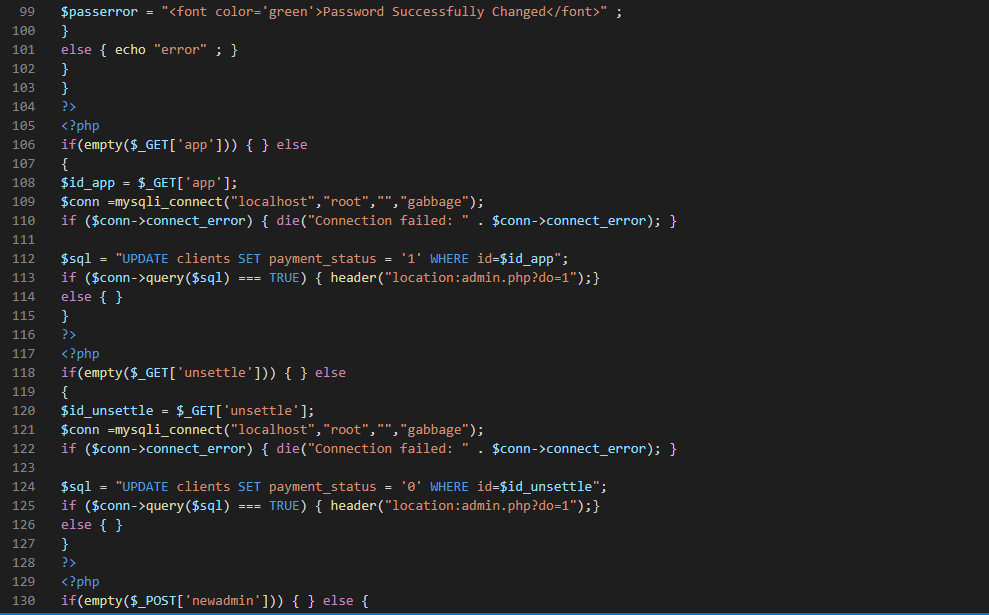
\includegraphics[width=0.8\textwidth]{ad4.png}
\end{figure}
\end{itemize}
\newpage
\newpage
\section{APPENDIX}
\subsection{\\QUESTIONAIRE}
Introduction and Consent:
\newline
\newline
Hallo, my name is.................................................. I am conducting a research on e-waste management on behalf of Nairobi county council. The research aims at reducing the levels of e-waste generation with emphasis on  proper disposal mechanism, strategies and system. This is realized by carrying out research, raising awareness and doing advocacy at all levels.
 I would like to ask you some questions related to how you manage your waste and its impact on the environment. Your answers to our questions will assist in assess the current situation and help in designing a system to manage emerging issues. Whatever you tell me is confidential and shall only be used for purposes of this study. If there are some questions that you do not wish to answer, just tell me and we will skip them. Do you have any questions? If yes, kindly clear the issues before proceeding with the interview.
Do you agree to participate? Yes/No.[.....] If No end interview and thank the interviewee.
\newline
\newline
 A. General\\
1. Date:............................................. Interviewer:................................................
\newline 2. Interviewee: .................................... Position:..........................................
\newline 3. Name of institution: ............................................................................
4. Type of institution:
\begin{itemize}
\item[$\square$] Government.
\item[$\square$]  Private co.
\item[$\square$]  NGO.
\item[$\square$] International.
\item[$\square$]   Informal busines
\end{itemize}
Other (Specify)................................................................

5. Type of stakeholder:
\begin{itemize}
\item[$\square$]Corporate consumer Individual consumer.
\item[$\square$]  Assembler Distributor
\item[$\square$] Importer Supplier                                  
\item[$\square$] Final disposer
\end{itemize}
Other (Specify).........................................................................................................

6. Is your institution ISO 140013 certified? 
\begin{itemize}
\item[$\square$]Yes.
\item[$\square$] No.
\end{itemize}
ISO 14001 is an internationally accepted standard that sets out how you can go
about putting in place an effective Environmental Management System (EMS). 

7. What brand of computers (desktop) do you deal with?
\begin{itemize}
\item[$\square$]IBM
\item[$\square$] Dell
\item[$\square$]HP                                  
\item[$\square$] Lenovo
\end{itemize}
Others (Specify)...............................................................................................

8. Are you aware that some hazardous fractions in e-waste need a special
treatment in order to be safely disposed of?
\begin{itemize}
\item[$\square$]Yes.
\item[$\square$] No.
\end{itemize}

 B. Customer\\

9. . Where did you acquire your equipment from?
\begin{itemize}
\item[$\square$]Retail outlet or shop
\item[$\square$] General distributor
\item[$\square$]Formal 2nd hand market
\item[$\square$]Informal 2nd hand market
\end{itemize}
Others, specify...................................................

10. What do you do with the equipment when it is no longer useful?
\begin{itemize}
\item[$\square$]Sell as 2nd hand equipment
\item[$\square$] Give them to a recycler
\item[$\square$]Donate to family, schools, employees, friends, etc.
\end{itemize}
Others, specify...............................................................

11.. For how long did you possess the equipment before you discarded (became
obsolete)?
\begin{itemize}
\item[$\square$]1 month-1 year
\item[$\square$] 1-2 years
\item[$\square$]4-5year
\item[$\square$]Over 5 years
\end{itemize}

12. In what condition was the equipment when you discarded it?
\begin{itemize}
\item[$\square$]Broken – unfixable
\item[$\square$] Broken – fixable
\item[$\square$]Working condition
\end{itemize}
Other, specify..................................................


13. Would you be ready to pay for your discarded equipment to be collected and
recycled?
\begin{itemize}
\item[$\square$]Yes.
\item[$\square$] No.
\end{itemize}

 C. E-waste collectors.

14. How do you identify the e-waste to be collected?..........................................................

15.How do you do the actual e-waste collection?
\begin{itemize}
\item[$\square$]Pick-up e-waste door to door?
\item[$\square$] Have a common collection point
\item[$\square$]Send municipal collection lorries
\item[$\square$]Pick from garbage disposal gardens
\end{itemize}
Others, specify...................................................................................................

16. Is the way e-waste is currently collected convenient to you?
\begin{itemize}
\item[$\square$]Yes.
\item[$\square$] No.
\end{itemize}

17. If no, what can be improved?
......................................................................

18. After collecting the e-waste, what do you do with it?
\begin{itemize}
\item[$\square$]Repair and sell as 2nd hand
\item[$\square$]Dismantle and sell as parts
\item[$\square$]Deposit to a refurbishing firm
\end{itemize}
Others, specify.............................................

\subsection{\\INTERVIEW}
 Interview with Ministry of Health.

1.How do you view e-waste management in kenya?

2.What effects does e-waste have in yuor ministry?

3.What kind of heal risks does e-waste pose to the community?

4.What opportunivies are available for you as a ministry in e-waste ?

5.Is there a need for e-waste policies and why?

6.Who should be incharge of formulating e-waste policies?

6.If and when the policy is formulate, what key factors should the policy cover?
\newline
 Interview with Ministry of Environment and Natural Resources.

1.How do you view e-waste management in kenya?

2.What effects does e-waste have in yuor ministry?

3.What kind of heal risks does e-waste pose to the community?

4.What opportunivies are available for you as a ministry in e-waste ?

5.Is there a need for e-waste policies and why?

6.Who should be incharge of formulating e-waste policies?

7.If and when the policy is formulate, what key factors should the policy cover?

\bibliographystyle{apacite}
\newpage
\bibliography{References}

\end{document}